\documentclass[11pt]{article}
\usepackage[T1]{fontenc}
% Nicer default font (+ math font) than Computer Modern for most use cases
\usepackage{mathpazo}

% Basic figure setup, for now with no caption control since it's done
% automatically by Pandoc (which extracts ![](path) syntax from Markdown).
\usepackage{graphicx}
% We will generate all images so they have a width \maxwidth. This means
% that they will get their normal width if they fit onto the page, but
% are scaled down if they would overflow the margins.
\makeatletter
% \def\maxwidth{\ifdim\Gin@nat@width>\linewidth\linewidth
% \else\Gin@nat@width\fi}
\makeatother
% \let\Oldincludegraphics\includegraphics
% Set max figure width to be 80% of text width, for now hardcoded.
%\renewcommand{\includegraphics}[1]{\Oldincludegraphics[width=.8\maxwidth]{#1}}
% Ensure that by default, figures have no caption (until we provide a
% proper Figure object with a Caption API and a way to capture that
% in the conversion process - todo).
\usepackage{caption}
\DeclareCaptionLabelFormat{nolabel}{}
\captionsetup{labelformat=nolabel}

\usepackage{adjustbox} % Used to constrain images to a maximum size 
\usepackage{xcolor} % Allow colors to be defined
\usepackage{enumerate} % Needed for markdown enumerations to work
% \usepackage{geometry} % Used to adjust the document margins
\usepackage{amsmath} % Equations
\usepackage{amssymb} % Equations
\usepackage{textcomp} % defines textquotesingle
% Hack from http://tex.stackexchange.com/a/47451/13684:
\AtBeginDocument{%
    \def\PYZsq{\textquotesingle}% Upright quotes in Pygmentized code
}
\usepackage{upquote} % Upright quotes for verbatim code
\usepackage{eurosym} % defines \euro
\usepackage[mathletters]{ucs} % Extended unicode (utf-8) support
\usepackage[utf8x]{inputenc} % Allow utf-8 characters in the tex document
\usepackage{fancyvrb} % verbatim replacement that allows latex
\usepackage{grffile} % extends the file name processing of package graphics 
                     % to support a larger range 
% The hyperref package gives us a pdf with properly built
% internal navigation ('pdf bookmarks' for the table of contents,
% internal cross-reference links, web links for URLs, etc.)
\usepackage{hyperref}
\usepackage{longtable} % longtable support required by pandoc >1.10
\usepackage{booktabs}  % table support for pandoc > 1.12.2
\usepackage[inline]{enumitem} % IRkernel/repr support (it uses the enumerate* environment)
\usepackage[normalem]{ulem} % ulem is needed to support strikethroughs (\sout)
                            % normalem makes italics be italics, not underlines


% Colors for the hyperref package
\definecolor{urlcolor}{rgb}{0,.145,.698}
\definecolor{linkcolor}{rgb}{.71,0.21,0.01}
\definecolor{citecolor}{rgb}{.12,.54,.11}

% ANSI colors
\definecolor{ansi-black}{HTML}{3E424D}
\definecolor{ansi-black-intense}{HTML}{282C36}
\definecolor{ansi-red}{HTML}{E75C58}
\definecolor{ansi-red-intense}{HTML}{B22B31}
\definecolor{ansi-green}{HTML}{00A250}
\definecolor{ansi-green-intense}{HTML}{007427}
\definecolor{ansi-yellow}{HTML}{DDB62B}
\definecolor{ansi-yellow-intense}{HTML}{B27D12}
\definecolor{ansi-blue}{HTML}{208FFB}
\definecolor{ansi-blue-intense}{HTML}{0065CA}
\definecolor{ansi-magenta}{HTML}{D160C4}
\definecolor{ansi-magenta-intense}{HTML}{A03196}
\definecolor{ansi-cyan}{HTML}{60C6C8}
\definecolor{ansi-cyan-intense}{HTML}{258F8F}
\definecolor{ansi-white}{HTML}{C5C1B4}
\definecolor{ansi-white-intense}{HTML}{A1A6B2}

% commands and environments needed by pandoc snippets
% extracted from the output of `pandoc -s`
\providecommand{\tightlist}{%
  \setlength{\itemsep}{0pt}\setlength{\parskip}{0pt}}
\DefineVerbatimEnvironment{Highlighting}{Verbatim}{commandchars=\\\{\}}
% Add ',fontsize=\small' for more characters per line
\newenvironment{Shaded}{}{}
\newcommand{\KeywordTok}[1]{\textcolor[rgb]{0.00,0.44,0.13}{\textbf{{#1}}}}
\newcommand{\DataTypeTok}[1]{\textcolor[rgb]{0.56,0.13,0.00}{{#1}}}
\newcommand{\DecValTok}[1]{\textcolor[rgb]{0.25,0.63,0.44}{{#1}}}
\newcommand{\BaseNTok}[1]{\textcolor[rgb]{0.25,0.63,0.44}{{#1}}}
\newcommand{\FloatTok}[1]{\textcolor[rgb]{0.25,0.63,0.44}{{#1}}}
\newcommand{\CharTok}[1]{\textcolor[rgb]{0.25,0.44,0.63}{{#1}}}
\newcommand{\StringTok}[1]{\textcolor[rgb]{0.25,0.44,0.63}{{#1}}}
\newcommand{\CommentTok}[1]{\textcolor[rgb]{0.38,0.63,0.69}{\textit{{#1}}}}
\newcommand{\OtherTok}[1]{\textcolor[rgb]{0.00,0.44,0.13}{{#1}}}
\newcommand{\AlertTok}[1]{\textcolor[rgb]{1.00,0.00,0.00}{\textbf{{#1}}}}
\newcommand{\FunctionTok}[1]{\textcolor[rgb]{0.02,0.16,0.49}{{#1}}}
\newcommand{\RegionMarkerTok}[1]{{#1}}
\newcommand{\ErrorTok}[1]{\textcolor[rgb]{1.00,0.00,0.00}{\textbf{{#1}}}}
\newcommand{\NormalTok}[1]{{#1}}

% Additional commands for more recent versions of Pandoc
\newcommand{\ConstantTok}[1]{\textcolor[rgb]{0.53,0.00,0.00}{{#1}}}
\newcommand{\SpecialCharTok}[1]{\textcolor[rgb]{0.25,0.44,0.63}{{#1}}}
\newcommand{\VerbatimStringTok}[1]{\textcolor[rgb]{0.25,0.44,0.63}{{#1}}}
\newcommand{\SpecialStringTok}[1]{\textcolor[rgb]{0.73,0.40,0.53}{{#1}}}
\newcommand{\ImportTok}[1]{{#1}}
\newcommand{\DocumentationTok}[1]{\textcolor[rgb]{0.73,0.13,0.13}{\textit{{#1}}}}
\newcommand{\AnnotationTok}[1]{\textcolor[rgb]{0.38,0.63,0.69}{\textbf{\textit{{#1}}}}}
\newcommand{\CommentVarTok}[1]{\textcolor[rgb]{0.38,0.63,0.69}{\textbf{\textit{{#1}}}}}
\newcommand{\VariableTok}[1]{\textcolor[rgb]{0.10,0.09,0.49}{{#1}}}
\newcommand{\ControlFlowTok}[1]{\textcolor[rgb]{0.00,0.44,0.13}{\textbf{{#1}}}}
\newcommand{\OperatorTok}[1]{\textcolor[rgb]{0.40,0.40,0.40}{{#1}}}
\newcommand{\BuiltInTok}[1]{{#1}}
\newcommand{\ExtensionTok}[1]{{#1}}
\newcommand{\PreprocessorTok}[1]{\textcolor[rgb]{0.74,0.48,0.00}{{#1}}}
\newcommand{\AttributeTok}[1]{\textcolor[rgb]{0.49,0.56,0.16}{{#1}}}
\newcommand{\InformationTok}[1]{\textcolor[rgb]{0.38,0.63,0.69}{\textbf{\textit{{#1}}}}}
\newcommand{\WarningTok}[1]{\textcolor[rgb]{0.38,0.63,0.69}{\textbf{\textit{{#1}}}}}

% Define a nice break command that doesn't care if a line doesn't already
% exist.
\def\br{\hspace*{\fill} \\* }
% Math Jax compatability definitions
\def\gt{>}
\def\lt{<}
% Document parameters
\title{Assignment \#3}

% Pygments definitions

\makeatletter
\def\PY@reset{\let\PY@it=\relax \let\PY@bf=\relax%
    \let\PY@ul=\relax \let\PY@tc=\relax%
    \let\PY@bc=\relax \let\PY@ff=\relax}
\def\PY@tok#1{\csname PY@tok@#1\endcsname}
\def\PY@toks#1+{\ifx\relax#1\empty\else%
    \PY@tok{#1}\expandafter\PY@toks\fi}
\def\PY@do#1{\PY@bc{\PY@tc{\PY@ul{%
    \PY@it{\PY@bf{\PY@ff{#1}}}}}}}
\def\PY#1#2{\PY@reset\PY@toks#1+\relax+\PY@do{#2}}

\expandafter\def\csname PY@tok@c\endcsname{\let\PY@it=\textit\def\PY@tc##1{\textcolor[rgb]{0.25,0.50,0.50}{##1}}}
\expandafter\def\csname PY@tok@vi\endcsname{\def\PY@tc##1{\textcolor[rgb]{0.10,0.09,0.49}{##1}}}
\expandafter\def\csname PY@tok@nc\endcsname{\let\PY@bf=\textbf\def\PY@tc##1{\textcolor[rgb]{0.00,0.00,1.00}{##1}}}
\expandafter\def\csname PY@tok@gs\endcsname{\let\PY@bf=\textbf}
\expandafter\def\csname PY@tok@gh\endcsname{\let\PY@bf=\textbf\def\PY@tc##1{\textcolor[rgb]{0.00,0.00,0.50}{##1}}}
\expandafter\def\csname PY@tok@il\endcsname{\def\PY@tc##1{\textcolor[rgb]{0.40,0.40,0.40}{##1}}}
\expandafter\def\csname PY@tok@fm\endcsname{\def\PY@tc##1{\textcolor[rgb]{0.00,0.00,1.00}{##1}}}
\expandafter\def\csname PY@tok@nf\endcsname{\def\PY@tc##1{\textcolor[rgb]{0.00,0.00,1.00}{##1}}}
\expandafter\def\csname PY@tok@mi\endcsname{\def\PY@tc##1{\textcolor[rgb]{0.40,0.40,0.40}{##1}}}
\expandafter\def\csname PY@tok@gr\endcsname{\def\PY@tc##1{\textcolor[rgb]{1.00,0.00,0.00}{##1}}}
\expandafter\def\csname PY@tok@c1\endcsname{\let\PY@it=\textit\def\PY@tc##1{\textcolor[rgb]{0.25,0.50,0.50}{##1}}}
\expandafter\def\csname PY@tok@ni\endcsname{\let\PY@bf=\textbf\def\PY@tc##1{\textcolor[rgb]{0.60,0.60,0.60}{##1}}}
\expandafter\def\csname PY@tok@bp\endcsname{\def\PY@tc##1{\textcolor[rgb]{0.00,0.50,0.00}{##1}}}
\expandafter\def\csname PY@tok@mb\endcsname{\def\PY@tc##1{\textcolor[rgb]{0.40,0.40,0.40}{##1}}}
\expandafter\def\csname PY@tok@ss\endcsname{\def\PY@tc##1{\textcolor[rgb]{0.10,0.09,0.49}{##1}}}
\expandafter\def\csname PY@tok@sx\endcsname{\def\PY@tc##1{\textcolor[rgb]{0.00,0.50,0.00}{##1}}}
\expandafter\def\csname PY@tok@sh\endcsname{\def\PY@tc##1{\textcolor[rgb]{0.73,0.13,0.13}{##1}}}
\expandafter\def\csname PY@tok@kp\endcsname{\def\PY@tc##1{\textcolor[rgb]{0.00,0.50,0.00}{##1}}}
\expandafter\def\csname PY@tok@vc\endcsname{\def\PY@tc##1{\textcolor[rgb]{0.10,0.09,0.49}{##1}}}
\expandafter\def\csname PY@tok@gd\endcsname{\def\PY@tc##1{\textcolor[rgb]{0.63,0.00,0.00}{##1}}}
\expandafter\def\csname PY@tok@gp\endcsname{\let\PY@bf=\textbf\def\PY@tc##1{\textcolor[rgb]{0.00,0.00,0.50}{##1}}}
\expandafter\def\csname PY@tok@gt\endcsname{\def\PY@tc##1{\textcolor[rgb]{0.00,0.27,0.87}{##1}}}
\expandafter\def\csname PY@tok@cs\endcsname{\let\PY@it=\textit\def\PY@tc##1{\textcolor[rgb]{0.25,0.50,0.50}{##1}}}
\expandafter\def\csname PY@tok@ne\endcsname{\let\PY@bf=\textbf\def\PY@tc##1{\textcolor[rgb]{0.82,0.25,0.23}{##1}}}
\expandafter\def\csname PY@tok@o\endcsname{\def\PY@tc##1{\textcolor[rgb]{0.40,0.40,0.40}{##1}}}
\expandafter\def\csname PY@tok@ch\endcsname{\let\PY@it=\textit\def\PY@tc##1{\textcolor[rgb]{0.25,0.50,0.50}{##1}}}
\expandafter\def\csname PY@tok@vg\endcsname{\def\PY@tc##1{\textcolor[rgb]{0.10,0.09,0.49}{##1}}}
\expandafter\def\csname PY@tok@si\endcsname{\let\PY@bf=\textbf\def\PY@tc##1{\textcolor[rgb]{0.73,0.40,0.53}{##1}}}
\expandafter\def\csname PY@tok@kt\endcsname{\def\PY@tc##1{\textcolor[rgb]{0.69,0.00,0.25}{##1}}}
\expandafter\def\csname PY@tok@kc\endcsname{\let\PY@bf=\textbf\def\PY@tc##1{\textcolor[rgb]{0.00,0.50,0.00}{##1}}}
\expandafter\def\csname PY@tok@kn\endcsname{\let\PY@bf=\textbf\def\PY@tc##1{\textcolor[rgb]{0.00,0.50,0.00}{##1}}}
\expandafter\def\csname PY@tok@cm\endcsname{\let\PY@it=\textit\def\PY@tc##1{\textcolor[rgb]{0.25,0.50,0.50}{##1}}}
\expandafter\def\csname PY@tok@ow\endcsname{\let\PY@bf=\textbf\def\PY@tc##1{\textcolor[rgb]{0.67,0.13,1.00}{##1}}}
\expandafter\def\csname PY@tok@nn\endcsname{\let\PY@bf=\textbf\def\PY@tc##1{\textcolor[rgb]{0.00,0.00,1.00}{##1}}}
\expandafter\def\csname PY@tok@vm\endcsname{\def\PY@tc##1{\textcolor[rgb]{0.10,0.09,0.49}{##1}}}
\expandafter\def\csname PY@tok@go\endcsname{\def\PY@tc##1{\textcolor[rgb]{0.53,0.53,0.53}{##1}}}
\expandafter\def\csname PY@tok@ge\endcsname{\let\PY@it=\textit}
\expandafter\def\csname PY@tok@sa\endcsname{\def\PY@tc##1{\textcolor[rgb]{0.73,0.13,0.13}{##1}}}
\expandafter\def\csname PY@tok@na\endcsname{\def\PY@tc##1{\textcolor[rgb]{0.49,0.56,0.16}{##1}}}
\expandafter\def\csname PY@tok@mo\endcsname{\def\PY@tc##1{\textcolor[rgb]{0.40,0.40,0.40}{##1}}}
\expandafter\def\csname PY@tok@s1\endcsname{\def\PY@tc##1{\textcolor[rgb]{0.73,0.13,0.13}{##1}}}
\expandafter\def\csname PY@tok@mf\endcsname{\def\PY@tc##1{\textcolor[rgb]{0.40,0.40,0.40}{##1}}}
\expandafter\def\csname PY@tok@sc\endcsname{\def\PY@tc##1{\textcolor[rgb]{0.73,0.13,0.13}{##1}}}
\expandafter\def\csname PY@tok@err\endcsname{\def\PY@bc##1{\setlength{\fboxsep}{0pt}\fcolorbox[rgb]{1.00,0.00,0.00}{1,1,1}{\strut ##1}}}
\expandafter\def\csname PY@tok@m\endcsname{\def\PY@tc##1{\textcolor[rgb]{0.40,0.40,0.40}{##1}}}
\expandafter\def\csname PY@tok@w\endcsname{\def\PY@tc##1{\textcolor[rgb]{0.73,0.73,0.73}{##1}}}
\expandafter\def\csname PY@tok@sr\endcsname{\def\PY@tc##1{\textcolor[rgb]{0.73,0.40,0.53}{##1}}}
\expandafter\def\csname PY@tok@cp\endcsname{\def\PY@tc##1{\textcolor[rgb]{0.74,0.48,0.00}{##1}}}
\expandafter\def\csname PY@tok@dl\endcsname{\def\PY@tc##1{\textcolor[rgb]{0.73,0.13,0.13}{##1}}}
\expandafter\def\csname PY@tok@no\endcsname{\def\PY@tc##1{\textcolor[rgb]{0.53,0.00,0.00}{##1}}}
\expandafter\def\csname PY@tok@nv\endcsname{\def\PY@tc##1{\textcolor[rgb]{0.10,0.09,0.49}{##1}}}
\expandafter\def\csname PY@tok@nd\endcsname{\def\PY@tc##1{\textcolor[rgb]{0.67,0.13,1.00}{##1}}}
\expandafter\def\csname PY@tok@se\endcsname{\let\PY@bf=\textbf\def\PY@tc##1{\textcolor[rgb]{0.73,0.40,0.13}{##1}}}
\expandafter\def\csname PY@tok@sb\endcsname{\def\PY@tc##1{\textcolor[rgb]{0.73,0.13,0.13}{##1}}}
\expandafter\def\csname PY@tok@kd\endcsname{\let\PY@bf=\textbf\def\PY@tc##1{\textcolor[rgb]{0.00,0.50,0.00}{##1}}}
\expandafter\def\csname PY@tok@nt\endcsname{\let\PY@bf=\textbf\def\PY@tc##1{\textcolor[rgb]{0.00,0.50,0.00}{##1}}}
\expandafter\def\csname PY@tok@gi\endcsname{\def\PY@tc##1{\textcolor[rgb]{0.00,0.63,0.00}{##1}}}
\expandafter\def\csname PY@tok@sd\endcsname{\let\PY@it=\textit\def\PY@tc##1{\textcolor[rgb]{0.73,0.13,0.13}{##1}}}
\expandafter\def\csname PY@tok@nl\endcsname{\def\PY@tc##1{\textcolor[rgb]{0.63,0.63,0.00}{##1}}}
\expandafter\def\csname PY@tok@nb\endcsname{\def\PY@tc##1{\textcolor[rgb]{0.00,0.50,0.00}{##1}}}
\expandafter\def\csname PY@tok@mh\endcsname{\def\PY@tc##1{\textcolor[rgb]{0.40,0.40,0.40}{##1}}}
\expandafter\def\csname PY@tok@s2\endcsname{\def\PY@tc##1{\textcolor[rgb]{0.73,0.13,0.13}{##1}}}
\expandafter\def\csname PY@tok@gu\endcsname{\let\PY@bf=\textbf\def\PY@tc##1{\textcolor[rgb]{0.50,0.00,0.50}{##1}}}
\expandafter\def\csname PY@tok@cpf\endcsname{\let\PY@it=\textit\def\PY@tc##1{\textcolor[rgb]{0.25,0.50,0.50}{##1}}}
\expandafter\def\csname PY@tok@s\endcsname{\def\PY@tc##1{\textcolor[rgb]{0.73,0.13,0.13}{##1}}}
\expandafter\def\csname PY@tok@k\endcsname{\let\PY@bf=\textbf\def\PY@tc##1{\textcolor[rgb]{0.00,0.50,0.00}{##1}}}
\expandafter\def\csname PY@tok@kr\endcsname{\let\PY@bf=\textbf\def\PY@tc##1{\textcolor[rgb]{0.00,0.50,0.00}{##1}}}

\def\PYZbs{\char`\\}
\def\PYZus{\char`\_}
\def\PYZob{\char`\{}
\def\PYZcb{\char`\}}
\def\PYZca{\char`\^}
\def\PYZam{\char`\&}
\def\PYZlt{\char`\<}
\def\PYZgt{\char`\>}
\def\PYZsh{\char`\#}
\def\PYZpc{\char`\%}
\def\PYZdl{\char`\$}
\def\PYZhy{\char`\-}
\def\PYZsq{\char`\'}
\def\PYZdq{\char`\"}
\def\PYZti{\char`\~}
% for compatibility with earlier versions
\def\PYZat{@}
\def\PYZlb{[}
\def\PYZrb{]}
\makeatother

% Exact colors from NB
\definecolor{incolor}{rgb}{0.0, 0.0, 0.5}
\definecolor{outcolor}{rgb}{0.545, 0.0, 0.0}


% Prevent overflowing lines due to hard-to-break entities
\sloppy 
% Setup hyperref package
\hypersetup{
  breaklinks=true,  % so long urls are correctly broken across lines
  colorlinks=true,
  urlcolor=urlcolor,
  linkcolor=linkcolor,
  citecolor=citecolor,
  }
% Slightly bigger margins than the latex defaults

% \geometry{verbose,tmargin=1in,bmargin=1in,lmargin=1in,rmargin=1in}

% No paragraph indentation
\setlength{\parindent}{0pt}
% For boxes around verbatim blocks
\usepackage{fancyvrb}
% For side-by-side-figures
\usepackage{subfig}
% Margins
\usepackage[margin=0.5in]{geometry}

\begin{document}

\maketitle

\begin{center}
	\textbf{COMP 4107 Fall 2017}
	
	\textbf{Basim Ramadhan 100 901 646}
	
	\textbf{Christian Abbott 100 863 049}
\end{center}

% \begin{center}\rule{0.5\linewidth}{\linethickness}\end{center}

\pagebreak

\section{Question 1}\label{question-1}

\subsection{Running Our Code}\label{running-our-code}

We have provided an easy-to-use Makefile to help you run our program:

\begin{Verbatim}[frame=single,commandchars=\\\{\}]
    \PY{n}{make} \PY{n}{prepare}\PY{o}{\PYZhy{}}\PY{n}{venv}
    \PY{o}{.}\PY{o}{/}\PY{n}{env}\PY{o}{/}\PY{n+nb}{bin}\PY{o}{/}\PY{n}{python} \PY{n}{hopfieldnet}\PY{o}{.}\PY{n}{py} \PY{l+m+mi}{2}
\end{Verbatim}

Otherwise, if you have matplotlib, numpy, and scikit-learn installed already:

\begin{Verbatim}[frame=single,commandchars=\\\{\}]
    \PY{c+c1}{\PYZsh{} Syntax}
    \PY{n}{python3} \PY{n}{hopfieldnet}\PY{o}{.}\PY{n}{py} \PY{n}{num\PYZus{}training\PYZus{}patterns}
    \PY{c+c1}{\PYZsh{} Example}
    \PY{n}{python3} \PY{n}{hopfieldnet}\PY{o}{.}\PY{n}{py} \PY{l+m+mi}{2}
\end{Verbatim}

Running the program will do the following:

\begin{enumerate}
	\def\labelenumi{\arabic{enumi}.}
	\tightlist
	\item Load the MNIST dataset using scikit-learn then subsample to only include 1's and 5's.
	\item Pick some random MNIST images to train with; quantity of images is user-defined using the \textbf{num\_training\_patterns} command-line parameter.
	\item Initialize a Hopfield network.
	\item Train the network using Storkey's learning rule.
	\item Degrade each training image with 20\% noise \textit{(flip 20\% of the image's bits)}.
	\item Test whether the network can restore the degraded images satisfactorily.
	\item Print out the network's recovery accuracy.
\end{enumerate}

After the program performs the above, it will display the following
visualizations:

\begin{enumerate}
	\def\labelenumi{\arabic{enumi}.}
	\tightlist
	\item The network's weights.
	\item The network's state \textit{(the sum of each neuron's own weights).}
	\item A comparison between each original image, its degraded version, and its recovered version.
\end{enumerate}

\subsection{Accuracy of Pattern Recovery / Classification}\label{accuracy-of-pattern-recovery-classification}

We experimented with the Hebb and Storkey learning rules for Hopfield
networks storing between 1 and 20 images. For each number of images
stored in the network, we repeated the experiment 20 times. In other
words, our experimentation was the following:

\begin{itemize}
\item
  Train on 1 image with Hebb's rule and test the network's
  recovery accuracy, 20 times.
\item
  Train on 2 images with Hebb's rule and test the network's
  recovery accuracy, 20 times.
\item
  \(\cdots\)
\item
  Train on 20 images with Hebb's rule and test the network's
  recovery accuracy, 20 times.
\item
  Train on 1 image with Storkey's rule and test the network's
  recovery accuracy, 20 times.
\item
  Train on 2 images with Storkey's rule and test the network's
  recovery accuracy, 20 times.
\item
  \(\cdots\)
\item
  Train on 20 images with Storkey's rule and test the network's
  recovery accuracy, 20 times.
\end{itemize}

\pagebreak

A few notes regarding our experiments:

\begin{itemize}
\item
  to degrade our images, we applied 20\% noise, which means that a random 20\%
  of the pattern's bits were flipped
\item
  the threshold for a recovery being considered a success was the
  following: the L2-norm between the original MNIST image and the recovered
  image must be less than 10. We found this threshold only lets very
  good recoveries pass
\end{itemize}

These experiments yields the accuracy values in the code and chart
below.

\subsubsection{Accuracy Chart}\label{accuracy-chart}

\begin{figure}[htbp]
	\centering
	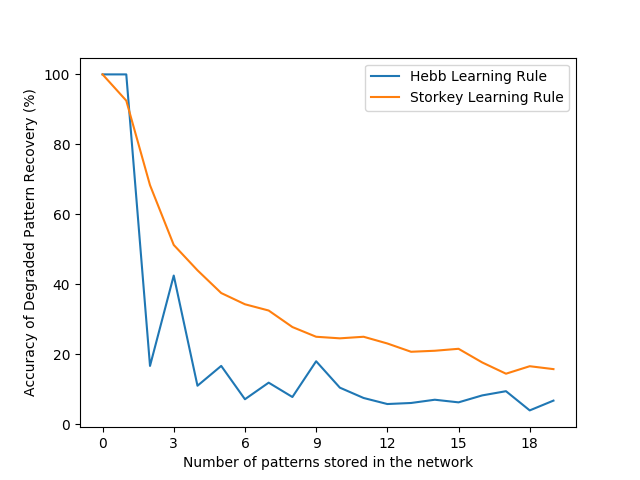
\includegraphics[scale=1.15]{../figures/q1/accuracy.png}
	\caption{Pattern Recovery Accuracy}
\end{figure}

\pagebreak

\subsubsection{Accuracy Chart Code}

Check out the accuracy values inside the code used to produce the previous chart:

\begin{Verbatim}[frame=single,commandchars=\\\{\}]
\PY{k+kn}{import} \PY{n+nn}{matplotlib}\PY{n+nn}{.}\PY{n+nn}{pyplot} \PY{k}{as} \PY{n+nn}{plt}
\PY{k+kn}{from} \PY{n+nn}{matplotlib}\PY{n+nn}{.}\PY{n+nn}{ticker} \PY{k}{import} \PY{n}{MaxNLocator}

\PY{n}{hebb\PYZus{}accuracy} \PY{o}{=} \PY{p}{[}
    \PY{l+m+mf}{100.00}\PY{p}{,} \PY{l+m+mf}{100.00}\PY{p}{,} \PY{l+m+mf}{16.67}\PY{p}{,} \PY{l+m+mf}{42.50}\PY{p}{,} \PY{l+m+mf}{11.00}\PY{p}{,}
    \PY{l+m+mf}{16.67}\PY{p}{,} \PY{l+m+mf}{7.14}\PY{p}{,} \PY{l+m+mf}{11.88}\PY{p}{,} \PY{l+m+mf}{7.78}\PY{p}{,} \PY{l+m+mf}{18.00}\PY{p}{,}
    \PY{l+m+mf}{10.45}\PY{p}{,} \PY{l+m+mf}{7.50}\PY{p}{,} \PY{l+m+mf}{5.77}\PY{p}{,} \PY{l+m+mf}{6.07}\PY{p}{,} \PY{l+m+mf}{7.00}\PY{p}{,}
    \PY{l+m+mf}{6.25}\PY{p}{,} \PY{l+m+mf}{8.24}\PY{p}{,} \PY{l+m+mf}{9.44}\PY{p}{,} \PY{l+m+mf}{3.95}\PY{p}{,} \PY{l+m+mf}{6.75}
\PY{p}{]}
\PY{n}{storkey\PYZus{}accuracy} \PY{o}{=} \PY{p}{[}
    \PY{l+m+mf}{100.00}\PY{p}{,} \PY{l+m+mf}{92.50}\PY{p}{,} \PY{l+m+mf}{68.33}\PY{p}{,} \PY{l+m+mf}{51.25}\PY{p}{,} \PY{l+m+mf}{44.00}\PY{p}{,}
    \PY{l+m+mf}{37.50}\PY{p}{,} \PY{l+m+mf}{34.29}\PY{p}{,} \PY{l+m+mf}{32.50}\PY{p}{,} \PY{l+m+mf}{27.78}\PY{p}{,} \PY{l+m+mf}{25.00}\PY{p}{,}
    \PY{l+m+mf}{24.55}\PY{p}{,} \PY{l+m+mf}{25.00}\PY{p}{,} \PY{l+m+mf}{23.08}\PY{p}{,} \PY{l+m+mf}{20.71}\PY{p}{,} \PY{l+m+mf}{21.00}\PY{p}{,}
    \PY{l+m+mf}{21.56}\PY{p}{,} \PY{l+m+mf}{17.65}\PY{p}{,} \PY{l+m+mf}{14.44}\PY{p}{,} \PY{l+m+mf}{16.58}\PY{p}{,} \PY{l+m+mf}{15.75}
\PY{p}{]}

\PY{n}{fig} \PY{o}{=} \PY{n}{plt}\PY{o}{.}\PY{n}{figure}\PY{p}{(}\PY{p}{)}
\PY{n}{ax} \PY{o}{=} \PY{n}{fig}\PY{o}{.}\PY{n}{gca}\PY{p}{(}\PY{p}{)}

\PY{n}{plt}\PY{o}{.}\PY{n}{plot}\PY{p}{(}\PY{n}{hebb\PYZus{}accuracy}\PY{p}{)}
\PY{n}{plt}\PY{o}{.}\PY{n}{plot}\PY{p}{(}\PY{n}{storkey\PYZus{}accuracy}\PY{p}{)}

\PY{n}{ax}\PY{o}{.}\PY{n}{xaxis}\PY{o}{.}\PY{n}{set\PYZus{}major\PYZus{}locator}\PY{p}{(}\PY{n}{MaxNLocator}\PY{p}{(}\PY{n}{integer}\PY{o}{=}\PY{k+kc}{True}\PY{p}{)}\PY{p}{)}
\PY{n}{plt}\PY{o}{.}\PY{n}{xlabel}\PY{p}{(}\PY{l+s+s2}{\PYZdq{}}\PY{l+s+s2}{Number of patterns stored in the network}\PY{l+s+s2}{\PYZdq{}}\PY{p}{)}
\PY{n}{plt}\PY{o}{.}\PY{n}{ylabel}\PY{p}{(}\PY{l+s+s2}{\PYZdq{}}\PY{l+s+s2}{Accuracy of Degraded Pattern Recovery (}\PY{l+s+s2}{\PYZpc{}}\PY{l+s+s2}{)}\PY{l+s+s2}{\PYZdq{}}\PY{p}{)}
\PY{n}{plt}\PY{o}{.}\PY{n}{legend}\PY{p}{(}\PY{p}{[}\PY{l+s+s1}{\PYZsq{}}\PY{l+s+s1}{Hebb Learning Rule}\PY{l+s+s1}{\PYZsq{}}\PY{p}{,} \PY{l+s+s1}{\PYZsq{}}\PY{l+s+s1}{Storkey Learning Rule}\PY{l+s+s1}{\PYZsq{}}\PY{p}{]}\PY{p}{,} \PY{n}{loc}\PY{o}{=}\PY{l+s+s1}{\PYZsq{}}\PY{l+s+s1}{upper right}\PY{l+s+s1}{\PYZsq{}}\PY{p}{)}

\PY{n}{plt}\PY{o}{.}\PY{n}{show}\PY{p}{(}\PY{p}{)}
\end{Verbatim}


\subsubsection{Analysis}\label{analysis}

Based on the data above---in addition to our experiences---we
have the following conclusions:

\begin{itemize}
% \tightlist
\item
  In general, training with Storkey's rule produces more accurate
  networks.
\item
  Hebb's rule surprisingly works better for 2-image networks than
  Storkey's rule.
\item
  Training with Hebb's rule (\textless{}1 second) is significantly
  faster than with Storkey's rule (\textasciitilde{}5 seconds).
\end{itemize}

\pagebreak

\subsection{Implementation}\label{implementation}

\subsubsection{Learning Rule
Implementations}\label{learning-rule-implementations}

For both learning rules, our initial implementations were simple and
followed their respective definitions closely. These implementations
were slow because they used nested for-loops with multiplications in
each iteration. We then implemented optimized versions of the learning
rules which used matrix operations instead. In the following code blocks
we show both unoptimized and optimized implementations.

\subsubsection{Hebb's Learning Rule}\label{hebbs-learning-rule}

\begin{Verbatim}[frame=single,commandchars=\\\{\}]
\PY{k}{def} \PY{n+nf}{train\PYZus{}hebbian}\PY{p}{(}\PY{n+nb+bp}{self}\PY{p}{,} \PY{n}{patterns}\PY{p}{)}\PY{p}{:}
    \PY{l+s+sd}{\PYZdq{}\PYZdq{}\PYZdq{}Train the Hopfield network using the Hebbian learning rule (1949).}
\PY{l+s+sd}{    https://en.wikipedia.org/wiki/Hopfield\PYZus{}network}
\PY{l+s+sd}{    \PYZdq{}\PYZdq{}\PYZdq{}}
    \PY{k}{for} \PY{n}{p} \PY{o+ow}{in} \PY{n}{patterns}\PY{p}{:}
        \PY{n}{a} \PY{o}{=} \PY{n}{p}\PY{o}{.}\PY{n}{reshape}\PY{p}{(}\PY{p}{(}\PY{n+nb+bp}{self}\PY{o}{.}\PY{n}{shape}\PY{p}{,} \PY{l+m+mi}{1}\PY{p}{)}\PY{p}{)}
        \PY{n}{b} \PY{o}{=} \PY{n}{a}\PY{o}{.}\PY{n}{T}
        \PY{n+nb+bp}{self}\PY{o}{.}\PY{n}{weights} \PY{o}{+}\PY{o}{=} \PY{n}{np}\PY{o}{.}\PY{n}{dot}\PY{p}{(}\PY{n}{a}\PY{p}{,} \PY{n}{b}\PY{p}{)}
    \PY{n+nb+bp}{self}\PY{o}{.}\PY{n}{weights} \PY{o}{\PYZhy{}}\PY{o}{=} \PY{p}{(}\PY{n}{np}\PY{o}{.}\PY{n}{identity}\PY{p}{(}\PY{n}{patterns}\PY{p}{[}\PY{l+m+mi}{0}\PY{p}{]}\PY{o}{.}\PY{n}{size}\PY{p}{)} \PY{o}{*} \PY{n}{patterns}\PY{o}{.}\PY{n}{shape}\PY{p}{[}\PY{l+m+mi}{0}\PY{p}{]}\PY{p}{)}
    \PY{k}{return} \PY{n+nb+bp}{self}\PY{o}{.}\PY{n}{weights}

\PY{k}{def} \PY{n+nf}{train\PYZus{}hebbian\PYZus{}unoptimized}\PY{p}{(}\PY{n+nb+bp}{self}\PY{p}{,} \PY{n}{patterns}\PY{p}{)}\PY{p}{:}
    \PY{l+s+sd}{\PYZdq{}\PYZdq{}\PYZdq{}Inefficient version of the train\PYZus{}hebbian function.}
\PY{l+s+sd}{    Performs individual multiplications instead of efficient matrix operations.\PYZdq{}\PYZdq{}\PYZdq{}}
    \PY{n}{n} \PY{o}{=} \PY{n+nb+bp}{self}\PY{o}{.}\PY{n}{shape}
    \PY{k}{for} \PY{n}{i}\PY{p}{,} \PY{n}{j} \PY{o+ow}{in} \PY{n}{itertools}\PY{o}{.}\PY{n}{product}\PY{p}{(}\PY{n+nb}{range}\PY{p}{(}\PY{n}{n}\PY{p}{)}\PY{p}{,} \PY{n+nb}{range}\PY{p}{(}\PY{n}{n}\PY{p}{)}\PY{p}{)}\PY{p}{:}
        \PY{n+nb+bp}{self}\PY{o}{.}\PY{n}{weights}\PY{p}{[}\PY{n}{i}\PY{p}{]}\PY{p}{[}\PY{n}{j}\PY{p}{]} \PY{o}{=} \PY{n+nb}{sum}\PY{p}{(}\PY{p}{[}\PY{n}{p}\PY{p}{[}\PY{n}{i}\PY{p}{]} \PY{o}{*} \PY{n}{p}\PY{p}{[}\PY{n}{j}\PY{p}{]} \PY{k}{for} \PY{n}{p} \PY{o+ow}{in} \PY{n}{patterns}\PY{p}{]}\PY{p}{)} \PY{o}{/} \PY{n}{n}
    \PY{k}{return} \PY{n+nb+bp}{self}\PY{o}{.}\PY{n}{weights}
\end{Verbatim}


\subsubsection{Storkey's Learning Rule}\label{storkeys-learning-rule}

\begin{Verbatim}[frame=single,commandchars=\\\{\}]
\PY{k}{def} \PY{n+nf}{train\PYZus{}storkey}\PY{p}{(}\PY{n+nb+bp}{self}\PY{p}{,} \PY{n}{patterns}\PY{p}{)}\PY{p}{:}
    \PY{l+s+sd}{\PYZdq{}\PYZdq{}\PYZdq{}Train the Hopfield network using the Storkey learning rule (1997).}
\PY{l+s+sd}{    https://en.wikipedia.org/wiki/Hopfield\PYZus{}network\PYZsh{}The\PYZus{}Storkey\PYZus{}learning\PYZus{}rule}
\PY{l+s+sd}{    \PYZdq{}\PYZdq{}\PYZdq{}}
    \PY{n}{n} \PY{o}{=} \PY{n+nb+bp}{self}\PY{o}{.}\PY{n}{shape}
    \PY{k}{for} \PY{n}{p} \PY{o+ow}{in} \PY{n}{patterns}\PY{p}{:}
        \PY{k}{for} \PY{n}{i}\PY{p}{,} \PY{n}{j} \PY{o+ow}{in} \PY{n}{itertools}\PY{o}{.}\PY{n}{product}\PY{p}{(}\PY{n+nb}{range}\PY{p}{(}\PY{n}{n}\PY{p}{)}\PY{p}{,} \PY{n+nb}{range}\PY{p}{(}\PY{n}{n}\PY{p}{)}\PY{p}{)}\PY{p}{:}
            \PY{n}{wt} \PY{o}{=} \PY{n+nb+bp}{self}\PY{o}{.}\PY{n}{weights}
            \PY{n}{w} \PY{o}{=} \PY{n}{wt}\PY{p}{[}\PY{n}{i}\PY{p}{]}\PY{p}{[}\PY{n}{j}\PY{p}{]}
            \PY{n}{x} \PY{o}{=} \PY{n}{p}\PY{p}{[}\PY{n}{i}\PY{p}{]} \PY{o}{*} \PY{n}{p}\PY{p}{[}\PY{n}{j}\PY{p}{]}
            \PY{n}{y} \PY{o}{=} \PY{n}{p}\PY{p}{[}\PY{n}{i}\PY{p}{]} \PY{o}{*} \PY{p}{(}\PY{n}{np}\PY{o}{.}\PY{n}{dot}\PY{p}{(}\PY{n}{wt}\PY{p}{[}\PY{n}{j}\PY{p}{]}\PY{p}{,} \PY{n}{p}\PY{p}{)} \PY{o}{\PYZhy{}} \PY{n}{wt}\PY{p}{[}\PY{n}{j}\PY{p}{]}\PY{p}{[}\PY{n}{i}\PY{p}{]} \PY{o}{*} \PY{n}{p}\PY{p}{[}\PY{n}{i}\PY{p}{]} \PY{o}{\PYZhy{}} \PY{n}{wt}\PY{p}{[}\PY{n}{j}\PY{p}{]}\PY{p}{[}\PY{n}{j}\PY{p}{]} \PY{o}{*} \PY{n}{p}\PY{p}{[}\PY{n}{j}\PY{p}{]}\PY{p}{)}
            \PY{n}{z} \PY{o}{=} \PY{n}{p}\PY{p}{[}\PY{n}{j}\PY{p}{]} \PY{o}{*} \PY{p}{(}\PY{n}{np}\PY{o}{.}\PY{n}{dot}\PY{p}{(}\PY{n}{wt}\PY{p}{[}\PY{n}{i}\PY{p}{]}\PY{p}{,} \PY{n}{p}\PY{p}{)} \PY{o}{\PYZhy{}} \PY{n}{wt}\PY{p}{[}\PY{n}{i}\PY{p}{]}\PY{p}{[}\PY{n}{i}\PY{p}{]} \PY{o}{*} \PY{n}{p}\PY{p}{[}\PY{n}{i}\PY{p}{]} \PY{o}{\PYZhy{}} \PY{n}{wt}\PY{p}{[}\PY{n}{i}\PY{p}{]}\PY{p}{[}\PY{n}{j}\PY{p}{]} \PY{o}{*} \PY{n}{p}\PY{p}{[}\PY{n}{j}\PY{p}{]}\PY{p}{)}
            \PY{n}{wt}\PY{p}{[}\PY{n}{i}\PY{p}{]}\PY{p}{[}\PY{n}{j}\PY{p}{]} \PY{o}{=} \PY{n}{w} \PY{o}{+} \PY{p}{(}\PY{p}{(}\PY{n}{x} \PY{o}{\PYZhy{}} \PY{n}{y} \PY{o}{\PYZhy{}} \PY{n}{z}\PY{p}{)} \PY{o}{/} \PY{n}{n}\PY{p}{)}


\PY{k}{def} \PY{n+nf}{train\PYZus{}storkey\PYZus{}unoptimized}\PY{p}{(}\PY{n+nb+bp}{self}\PY{p}{,} \PY{n}{patterns}\PY{p}{)}\PY{p}{:}
    \PY{l+s+sd}{\PYZdq{}\PYZdq{}\PYZdq{}Inefficient version of the train\PYZus{}storkey function.}
\PY{l+s+sd}{    Performs individual multiplications instead of efficient matrix operations.\PYZdq{}\PYZdq{}\PYZdq{}}
    \PY{n}{n} \PY{o}{=} \PY{n+nb+bp}{self}\PY{o}{.}\PY{n}{shape}
    \PY{k}{for} \PY{n}{p} \PY{o+ow}{in} \PY{n}{patterns}\PY{p}{:}
        \PY{k}{for} \PY{n}{i}\PY{p}{,} \PY{n}{j} \PY{o+ow}{in} \PY{n}{itertools}\PY{o}{.}\PY{n}{product}\PY{p}{(}\PY{n+nb}{range}\PY{p}{(}\PY{n}{n}\PY{p}{)}\PY{p}{,} \PY{n+nb}{range}\PY{p}{(}\PY{n}{n}\PY{p}{)}\PY{p}{)}\PY{p}{:}
            \PY{n}{w} \PY{o}{=} \PY{n+nb+bp}{self}\PY{o}{.}\PY{n}{weights}\PY{p}{[}\PY{n}{i}\PY{p}{]}\PY{p}{[}\PY{n}{j}\PY{p}{]}
            \PY{n}{x} \PY{o}{=} \PY{n}{p}\PY{p}{[}\PY{n}{i}\PY{p}{]} \PY{o}{*} \PY{n}{p}\PY{p}{[}\PY{n}{j}\PY{p}{]} \PY{o}{/} \PY{n}{n}
            \PY{n}{y} \PY{o}{=} \PY{n}{p}\PY{p}{[}\PY{n}{i}\PY{p}{]} \PY{o}{*} \PY{n+nb}{sum}\PY{p}{(}\PY{p}{[}\PY{n}{w}\PY{p}{[}\PY{n}{j}\PY{p}{]}\PY{p}{[}\PY{n}{k}\PY{p}{]} \PY{o}{*} \PY{n}{p}\PY{p}{[}\PY{n}{k}\PY{p}{]} \PY{k}{for} \PY{n}{k} \PY{o+ow}{in} \PY{n+nb}{range}\PY{p}{(}\PY{n}{n}\PY{p}{)} \PY{k}{if} \PY{n}{k} \PY{o+ow}{not} \PY{o+ow}{in} \PY{p}{[}\PY{n}{i}\PY{p}{,} \PY{n}{j}\PY{p}{]}\PY{p}{]}\PY{p}{)} \PY{o}{/} \PY{n}{n}
            \PY{n}{z} \PY{o}{=} \PY{n}{p}\PY{p}{[}\PY{n}{j}\PY{p}{]} \PY{o}{*} \PY{n+nb}{sum}\PY{p}{(}\PY{p}{[}w\PY{p}{[}\PY{n}{i}\PY{p}{]}\PY{p}{[}\PY{n}{k}\PY{p}{]} \PY{o}{*} \PY{n}{p}\PY{p}{[}\PY{n}{k}\PY{p}{]} \PY{k}{for} \PY{n}{k} \PY{o+ow}{in} \PY{n+nb}{range}\PY{p}{(}\PY{n}{n}\PY{p}{)} \PY{k}{if} \PY{n}{k} \PY{o+ow}{not} \PY{o+ow}{in} \PY{p}{[}\PY{n}{i}\PY{p}{,} \PY{n}{j}\PY{p}{]}\PY{p}{]}\PY{p}{)} \PY{o}{/} \PY{n}{n}
            \PY{n}{w}\PY{p}{[}\PY{n}{i}\PY{p}{]}\PY{p}{[}\PY{n}{j}\PY{p}{]} \PY{o}{=} \PY{n}{w} \PY{o}{+} \PY{n}{x} \PY{o}{\PYZhy{}} \PY{n}{y} \PY{o}{\PYZhy{}} \PY{n}{z}
\end{Verbatim}


    \subsubsection{Activation}\label{activation}

Our activation function follows the definition on the Wikipedia page.

\begin{Verbatim}[frame=single,commandchars=\\\{\}]
\PY{k}{def} \PY{n+nf}{activate}\PY{p}{(}\PY{n+nb+bp}{self}\PY{p}{,} \PY{n}{i}\PY{p}{)}\PY{p}{:}
    \PY{l+s+sd}{\PYZdq{}\PYZdq{}\PYZdq{}Determine whether the given neuron should be active or inactive.}
\PY{l+s+sd}{    https://en.wikipedia.org/wiki/Hopfield\PYZus{}network\PYZsh{}Updating\PYZdq{}\PYZdq{}\PYZdq{}}
    \PY{n}{weight\PYZus{}sum} \PY{o}{=} \PY{n}{np}\PY{o}{.}\PY{n}{dot}\PY{p}{(}\PY{n+nb+bp}{self}\PY{o}{.}\PY{n}{weights}\PY{p}{[}\PY{n}{i}\PY{p}{]}\PY{p}{,} \PY{n+nb+bp}{self}\PY{o}{.}\PY{n}{state}\PY{p}{)}
    \PY{n+nb+bp}{self}\PY{o}{.}\PY{n}{state}\PY{p}{[}\PY{n}{i}\PY{p}{]} \PY{o}{=} \PY{l+m+mi}{1} \PY{k}{if} \PY{n}{weight\PYZus{}sum} \PY{o}{\PYZgt{}} \PY{n+nb+bp}{self}\PY{o}{.}\PY{n}{thresholds}\PY{p}{[}\PY{n}{i}\PY{p}{]} \PY{k}{else} \PY{o}{\PYZhy{}}\PY{l+m+mi}{1}

\PY{k}{def} \PY{n+nf}{activate\PYZus{}unoptimized}\PY{p}{(}\PY{n+nb+bp}{self}\PY{p}{,} \PY{n}{i}\PY{p}{)}\PY{p}{:}
    \PY{l+s+sd}{\PYZdq{}\PYZdq{}\PYZdq{}Inefficient version of activate.\PYZdq{}\PYZdq{}\PYZdq{}}
    \PY{n}{num\PYZus{}neurons} \PY{o}{=} \PY{n+nb+bp}{self}\PY{o}{.}\PY{n}{shape}
    \PY{n}{weight\PYZus{}sum} \PY{o}{=} \PY{l+m+mf}{0.0}
    \PY{k}{for} \PY{n}{j} \PY{o+ow}{in} \PY{n+nb}{range}\PY{p}{(}\PY{n}{num\PYZus{}neurons}\PY{p}{)}\PY{p}{:}
        \PY{n}{weight\PYZus{}sum} \PY{o}{+}\PY{o}{=} \PY{n+nb+bp}{self}\PY{o}{.}\PY{n}{weights}\PY{p}{[}\PY{n}{i}\PY{p}{]}\PY{p}{[}\PY{n}{j}\PY{p}{]} \PY{o}{*} \PY{n+nb+bp}{self}\PY{o}{.}\PY{n}{state}\PY{p}{[}\PY{n}{j}\PY{p}{]}
    \PY{n+nb+bp}{self}\PY{o}{.}\PY{n}{state}\PY{p}{[}\PY{n}{i}\PY{p}{]} \PY{o}{=} \PY{l+m+mi}{1} \PY{k}{if} \PY{n}{weight\PYZus{}sum} \PY{o}{\PYZgt{}} \PY{n+nb+bp}{self}\PY{o}{.}\PY{n}{thresholds}\PY{p}{[}\PY{n}{i}\PY{p}{]} \PY{k}{else} \PY{o}{\PYZhy{}}\PY{l+m+mi}{1}
\end{Verbatim}


\subsubsection{Recovery}\label{recovery}

We took our own approach to recovering degraded patterns. At each
iteration, we call activate on each neuron in random order. If no state
changes take place during a single iteration, then the network state is
stable the image has (hopefully) been recovered. If the network is not
stable yet, we repeat for another iteration.

\begin{Verbatim}[frame=single,commandchars=\\\{\}]
\PY{k}{def} \PY{n+nf}{restore}\PY{p}{(}\PY{n+nb+bp}{self}\PY{p}{,} \PY{n}{degraded\PYZus{}pattern}\PY{p}{)}\PY{p}{:}
    \PY{l+s+sd}{\PYZdq{}\PYZdq{}\PYZdq{}Recover the original pattern of the degraded input pattern.\PYZdq{}\PYZdq{}\PYZdq{}}
    \PY{n+nb+bp}{self}\PY{o}{.}\PY{n}{state} \PY{o}{=} \PY{n}{np}\PY{o}{.}\PY{n}{copy}\PY{p}{(}\PY{n}{degraded\PYZus{}pattern}\PY{p}{)}
    \PY{n}{num\PYZus{}neurons} \PY{o}{=} \PY{n+nb+bp}{self}\PY{o}{.}\PY{n}{shape}

    \PY{c+c1}{\PYZsh{} During each iteration: ensure each neuron is activated at least once}
    \PY{n}{iterations} \PY{o}{=} \PY{l+m+mi}{0}
    \PY{k}{while} \PY{n}{iterations} \PY{o}{\PYZlt{}} \PY{l+m+mi}{10}\PY{p}{:}
        \PY{n}{changed} \PY{o}{=} \PY{k+kc}{False}
        \PY{n}{neurons} \PY{o}{=} \PY{n+nb}{list}\PY{p}{(}\PY{n+nb}{range}\PY{p}{(}\PY{n}{num\PYZus{}neurons}\PY{p}{)}\PY{p}{)}
        \PY{n}{random}\PY{o}{.}\PY{n}{shuffle}\PY{p}{(}\PY{n}{neurons}\PY{p}{)}
        \PY{k}{while} \PY{n}{neurons}\PY{p}{:}
            \PY{n}{neuron} \PY{o}{=} \PY{n}{neurons}\PY{o}{.}\PY{n}{pop}\PY{p}{(}\PY{p}{)}
            \PY{n}{old\PYZus{}state} \PY{o}{=} \PY{n+nb+bp}{self}\PY{o}{.}\PY{n}{state}\PY{p}{[}\PY{n}{neuron}\PY{p}{]}
            \PY{n+nb+bp}{self}\PY{o}{.}\PY{n}{activate}\PY{p}{(}\PY{n}{neuron}\PY{p}{)}
            \PY{n}{new\PYZus{}state} \PY{o}{=} \PY{n+nb+bp}{self}\PY{o}{.}\PY{n}{state}\PY{p}{[}\PY{n}{neuron}\PY{p}{]}
            \PY{n}{changed} \PY{o}{=} \PY{k+kc}{True} \PY{k}{if} \PY{n}{old\PYZus{}state} \PY{o}{!=} \PY{n}{new\PYZus{}state} \PY{k}{else} \PY{n}{changed}
        \PY{n}{iterations} \PY{o}{+}\PY{o}{=} \PY{l+m+mi}{1}
        \PY{k}{if} \PY{o+ow}{not} \PY{n}{changed}\PY{p}{:}
            \PY{k}{break}

    \PY{n}{recovered\PYZus{}pattern} \PY{o}{=} \PY{n}{np}\PY{o}{.}\PY{n}{copy}\PY{p}{(}\PY{n+nb+bp}{self}\PY{o}{.}\PY{n}{state}\PY{p}{)}
    \PY{k}{return} \PY{n}{recovered\PYZus{}pattern}
\end{Verbatim}

\pagebreak

\subsection{Pattern Recovery Visualizations}\label{pattern-recovery-visualizations}

\subsubsection{Successful Recovery from a 2-image Hebb-trained Network}\label{recovery-from-hebb-trained-networks}

\begin{figure}[h!]
	\centering
	\subfloat[Recovering a 5]{{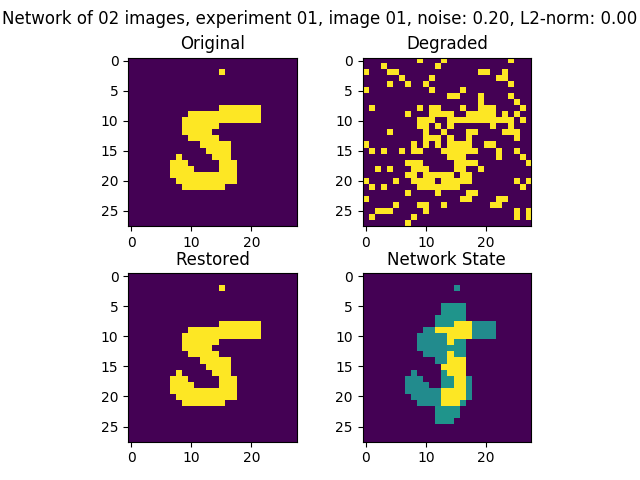
\includegraphics[width=9cm]{../figures/q1/hebb-recovery-01.png} }}
	\qquad
	\subfloat[Recovering a 1]{{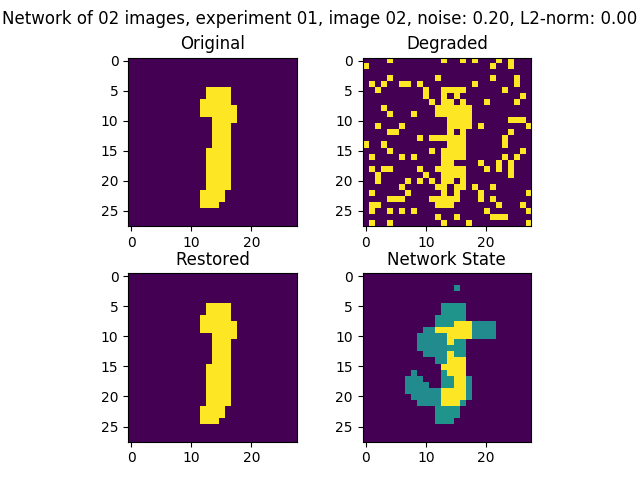
\includegraphics[width=9cm]{../figures/q1/hebb-recovery-02.png} }}
	\caption{Recovering from a 2-image Hebb-trained network}
\end{figure}

\subsubsection{Failed Recovery from a 9-image Hebb-trained Network}

\begin{figure}[h!]
	\centering
	\subfloat[Failing to recover a 5]{{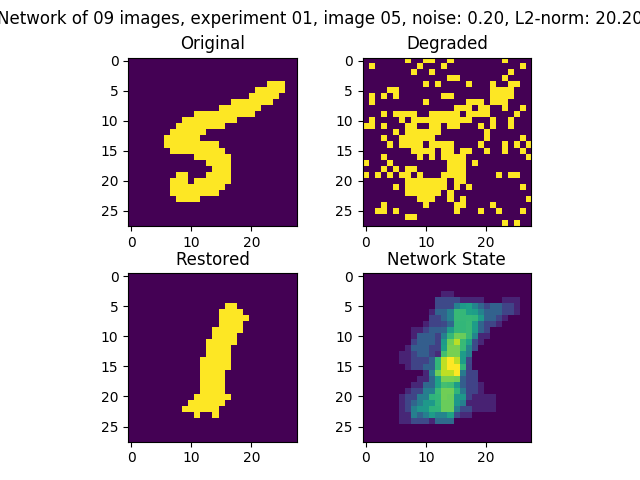
\includegraphics[width=9cm]{../figures/q1/hebb-recovery-03.png} }}
	\qquad
	\subfloat[Failing to recover a 5, again]{{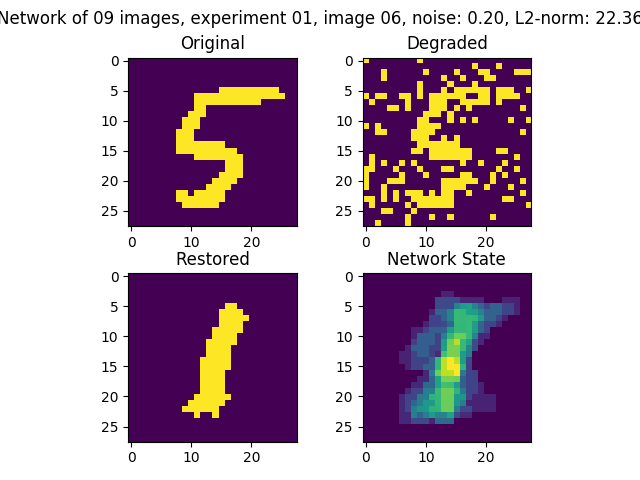
\includegraphics[width=9cm]{../figures/q1/hebb-recovery-04.png} }}
	\caption{Failing to recover from a 9-image Hebb-trained  network}
\end{figure}

\pagebreak

\subsubsection{Successful Recovery from Storkey-trained Networks}

\begin{figure}[h!]
	\centering
	\subfloat[Recovering a 5]{{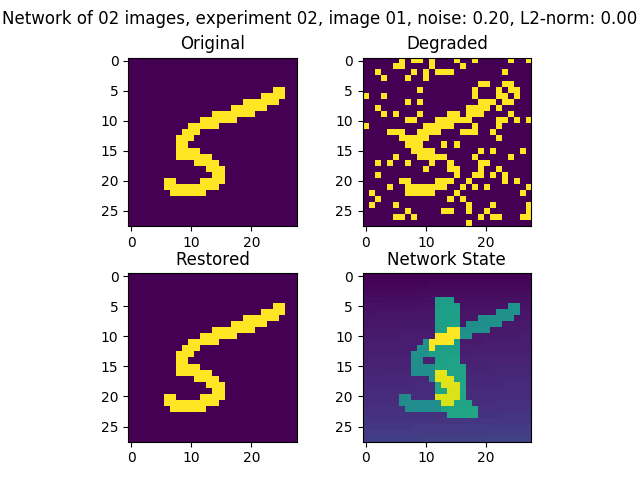
\includegraphics[width=9cm]{../figures/q1/storkey-recovery-01.png} }}
	\qquad
	\subfloat[Recovering a 1]{{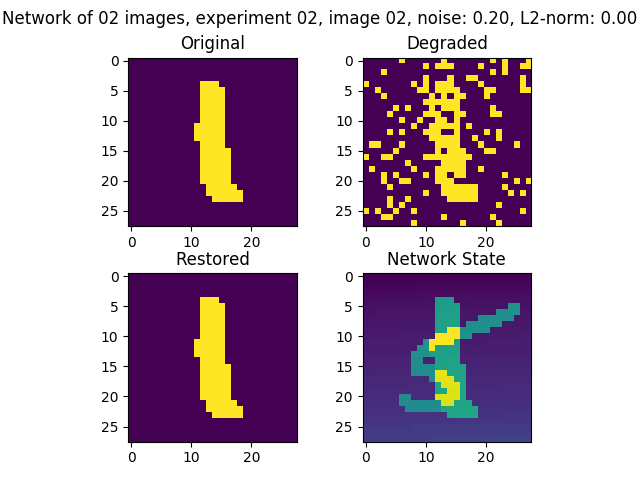
\includegraphics[width=9cm]{../figures/q1/storkey-recovery-02.png} }}
	\caption{Recovering from a 2-image Storkey-trained network}
\end{figure}

\begin{figure}[h!]
	\centering
	\subfloat[Recovering a 1]{{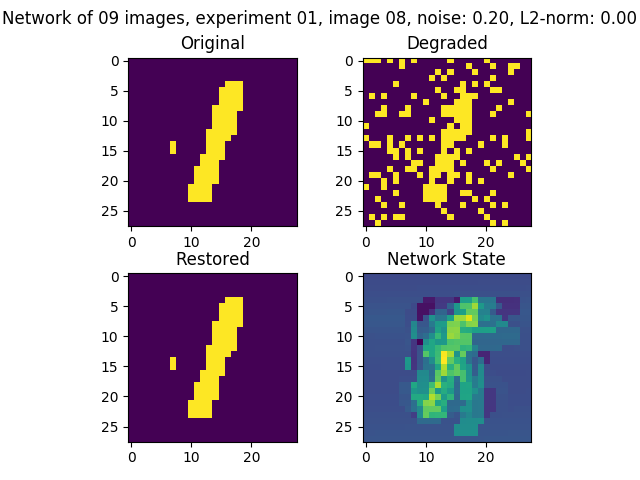
\includegraphics[width=9cm]{../figures/q1/storkey-recovery-03.png} }}
	\qquad
	\subfloat[Recovering a 1]{{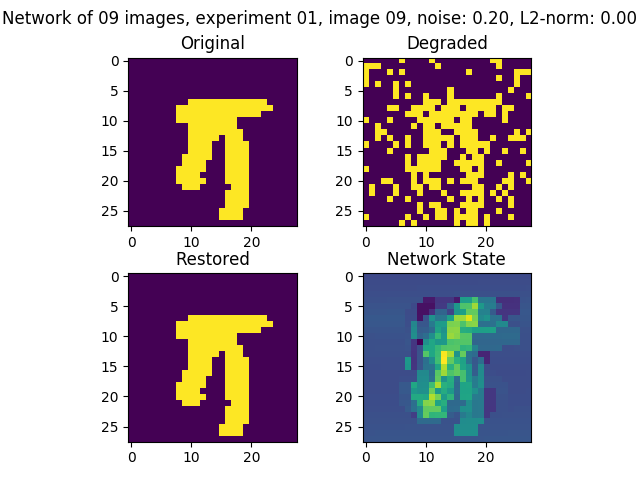
\includegraphics[width=9cm]{../figures/q1/storkey-recovery-04.png} }}
	\caption{Recovering from a 9-image Storkey-trained network}
\end{figure}

\pagebreak

\subsubsection{Failed Recovery from Storkey-trained Networks}

\begin{figure}[h!]
	\centering
	\subfloat[Failing to recover a 5]{{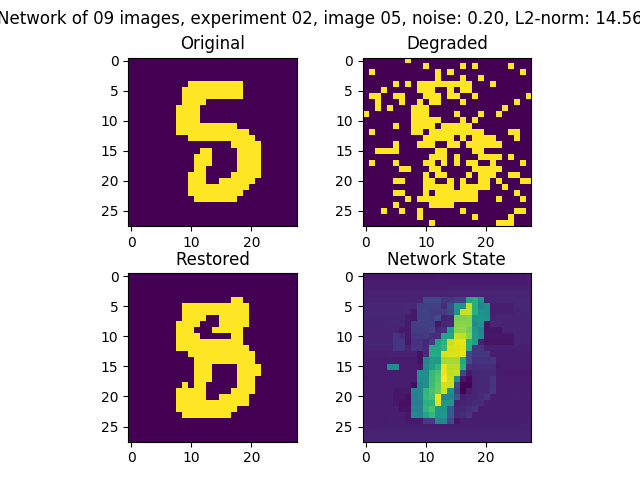
\includegraphics[width=9cm]{../figures/q1/storkey-recovery-05.png} }}
	\qquad
	\subfloat[Failing to recover a 5, again]{{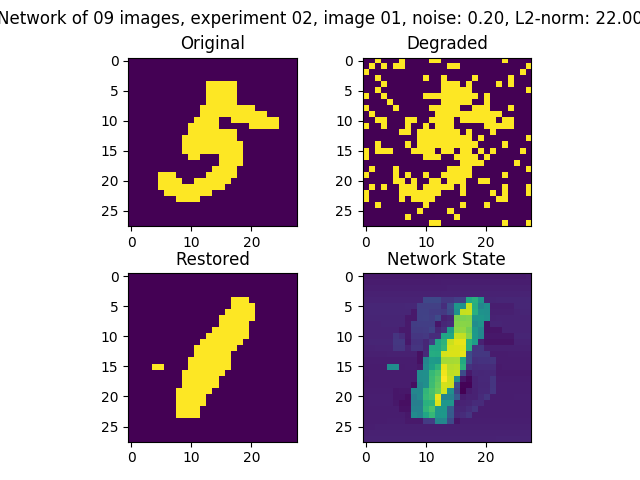
\includegraphics[width=9cm]{../figures/q1/storkey-recovery-06.png} }}
	\caption{Failing to recover from a 9-image Storkey-trained network}
\end{figure}

\pagebreak

\subsection{Network Visualizations}\label{network-visualizations}

We visualized our Hopfield networks after training them. We did this to
get a better understanding of how the and Hebb and Storkey learning
rules affect the network. We found that Hebb's rule produced a simpler,
less-detailed network; conversely, Storkey's rules produced a more nuanced network.
\\

You can see this in the diagrams that follow: in Hebb-trained networks,
the visualizations use fewer colors; this means that there's less
information in the network. Meanwhile in Storkey-trained networks, the
presence of more shades of color indicate a nuanced, more detailed
network.
\\

Furthermore, it's also interesting to visually see patterns stored in
the network in the "Network State" visualizations. We did this
visualization by summing the weights of each neuron to decide on the
color; then plotting a 28x28 grid of neurons with their respective
colors.
\\

In both examples, the same two patterns were used to train the networks.

\begin{figure}[h!]
	\centering
	\begin{tabular}{cc}
		\subfloat[Hebb Network Weights]{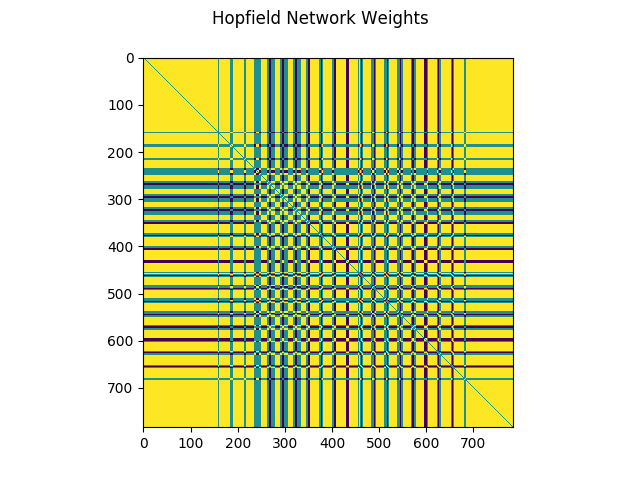
\includegraphics[scale=0.55]{../figures/q1/hebb-network-weights.png}} &
		\subfloat[Hebb Network State]{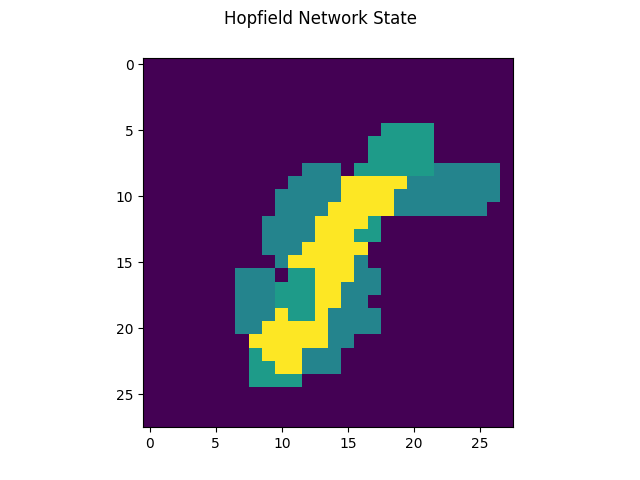
\includegraphics[scale=0.55]{../figures/q1/hebb-network-state.png}}
		\\
		\subfloat[Storkey Network Weight]{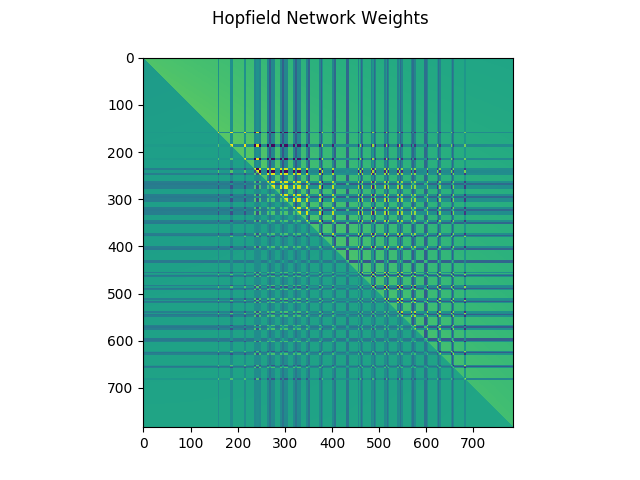
\includegraphics[scale=0.55]{../figures/q1/storkey-network-weights.png}} &
		\subfloat[Storkey Network State]{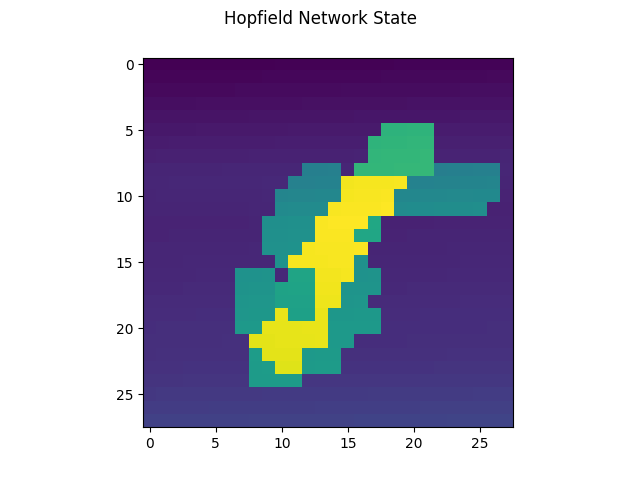
\includegraphics[scale=0.55]{../figures/q1/storkey-network-state.png}}
	\end{tabular}
\end{figure}

\begin{center}\rule{0.5\linewidth}{\linethickness}\end{center}

\pagebreak


\section{Question 2}\label{question-2}

\subsection{Running Our Code}\label{running-our-code}

We have provided an easy-to-use Makefile to help you run our program:

\begin{Verbatim}[frame=single,commandchars=\\\{\}]
    \PY{n}{make} \PY{n}{prepare}\PY{o}{\PYZhy{}}\PY{n}{venv}
    \PY{o}{.}\PY{o}{/}\PY{n}{env}\PY{o}{/}\PY{n+nb}{bin}\PY{o}{/}\PY{n}{python} \PY{n}{som}\PY{o}{.}\PY{n}{py}
\end{Verbatim}

Otherwise, if you have tensorflow, matplotlib, numpy, and scikit-learn
installed already:

\begin{Verbatim}[frame=single,commandchars=\\\{\}]
    \PY{n}{python3} \PY{n}{som}\PY{o}{.}\PY{n}{py}
\end{Verbatim}


Running the program will do the following:

\begin{enumerate}
	\tightlist
	 \item Fetch MNIST data and retrieve the 1's and 5's; this will be our dataset.
	 \item Initialize the SOM and train it on a subset of the dataset from step 1, in random order without replacement.
	 \item Test the clustering accuracy of the trained SOM and print out the value.
	 \item Perform K-means clustering on the dataset reduced to 2 dimensions.
	 \item Test the clustering accuracy of the K-means clustering and print out the value.
\end{enumerate}

After the programs performs the above, it will display three visualizations:

\begin{itemize}
	\tightlist
	\item The state of the SOM upon initialization.
	\item The state of the SOM after training.
	\item The K-means clustering of the dataset.
\end{itemize}


\subsection{Accuracy of Clustering}\label{accuracy-of-clustering}

When you run our program it will print out the clustering accuracies of
our trained SOM as well as our K-means output. We got the following
accuracy values:

\begin{itemize}
	\tightlist
	\item \textbf{SOM clustering accuracy: 94.80\%}
	\item \textbf{K-means clustering accuracy: 90.94\%}
\end{itemize}

    \subsection{SOM Dimensions}\label{som-dimensions}

In our implementation of an SOM, we used the following architecture:

\begin{itemize}
\tightlist
\item
  \textbf{Input layer:} 784 neurons / features
\item
  \textbf{Output layer:} 900 neurons
\end{itemize}

In our implementation, we found it useful to consider the output layer
as a 30x30 grid of neurons. Note that this is identical to saying we
used 900 output neurons.

    \subsection{SOM Parameters}\label{som-parameters}

We used the following parameters for our SOM implementation:

\begin{itemize}
	\tightlist
	\item Learning rate: $0.5$
	\item sigma (\(\sigma\)): 5.0 \ \textit{(for the Gaussian that updates the winner neuron's neighbours)}
	\item Number of input neurons: 784
	\item Number of output neurons: 900
\end{itemize}

For our weights, we initialized them according to a normal distribution
with \(\mu = 0.5\) and \(\sigma = 1.0\).

\pagebreak

\subsection{Visualizations}\label{visualizations}

\subsubsection{SOM Network}\label{som-network}

\begin{figure}[h!]
	\centering
	\subfloat[Before Training]{{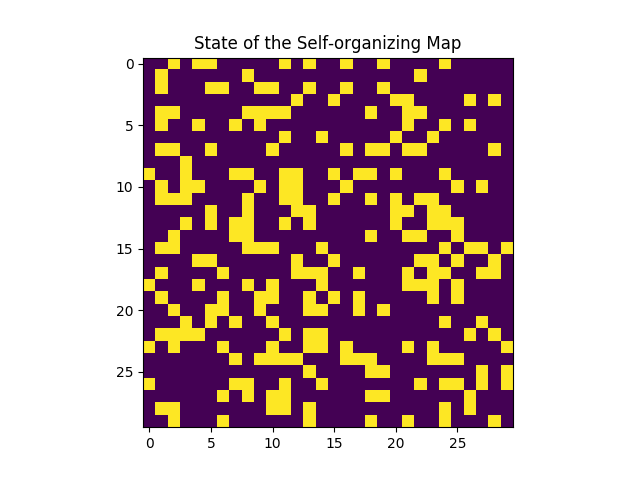
\includegraphics[width=14cm]{../figures/q2/som-network-state-before-training.png} }}
	\qquad
	\subfloat[After Training]{{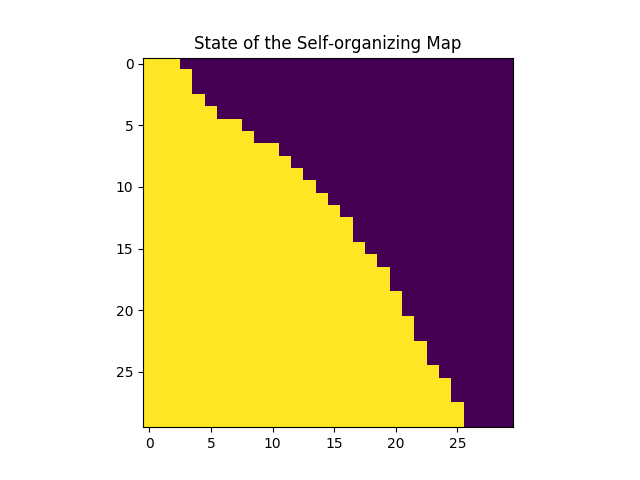
\includegraphics[width=14cm]{../figures/q2/som-network-state-after-training.png} }}
	\caption{The SOM Network Before \& After Training}
\end{figure}

\subsubsection{SOM Training Process}\label{som-training-process}

We were interested in visualizing the SOM's training process. We created
visualizations after each training iteration to see how the SOM changes
over time. We start off in the top left with random weights.
\\

We progressively train with MNIST images until, at iteration 15 (bottom
right) we have a clear partitioning of the map into two partitions.
Training any more just makes the map dance around more, not improving
the map very much.
\\

The purple partition represents MNIST images of the number 1. The yellow
partition represent MNIST images of the number 5.

\begin{figure}[h!]
	\begin{tabular}{cccc}
		\subfloat[Iteration 0]{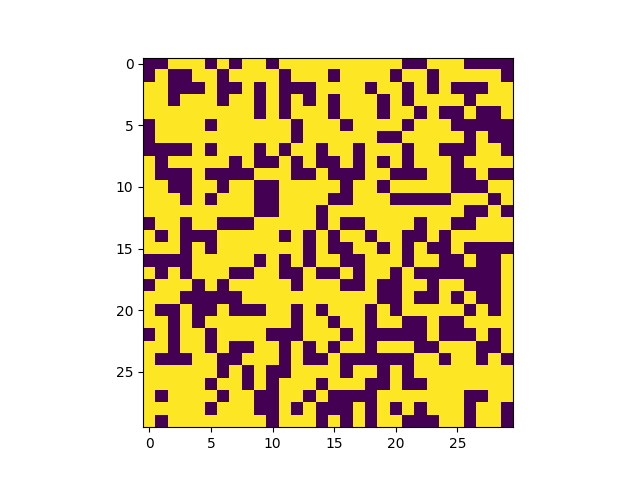
\includegraphics[width = 1.7in]{../figures/q2/som-training-00.png}} &
		\subfloat[Iteration 1]{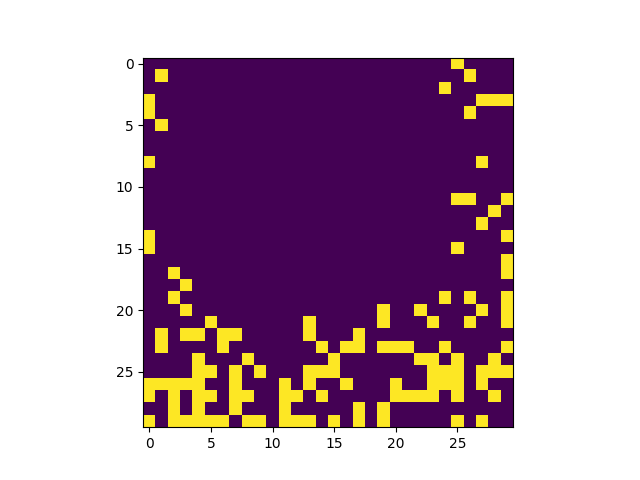
\includegraphics[width = 1.7in]{../figures/q2/som-training-01.png}} &
		\subfloat[Iteration 2]{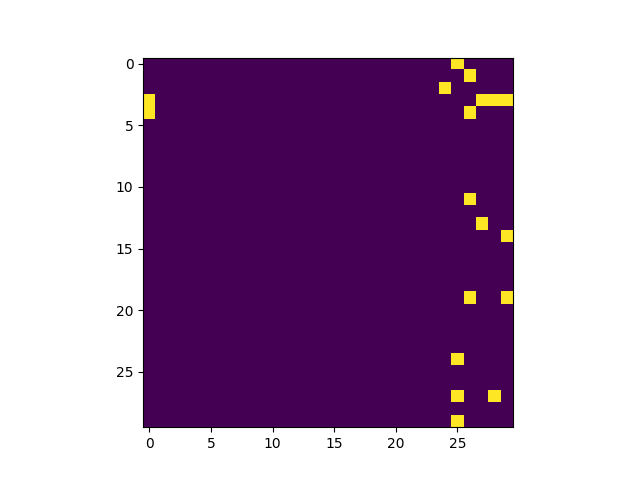
\includegraphics[width = 1.7in]{../figures/q2/som-training-02.png}} &
		\subfloat[Iteration 3]{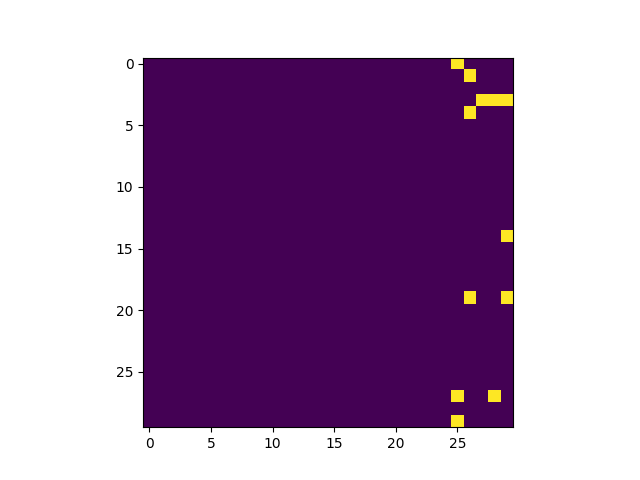
\includegraphics[width = 1.7in]{../figures/q2/som-training-03.png}}\\
		\subfloat[Iteration 4]{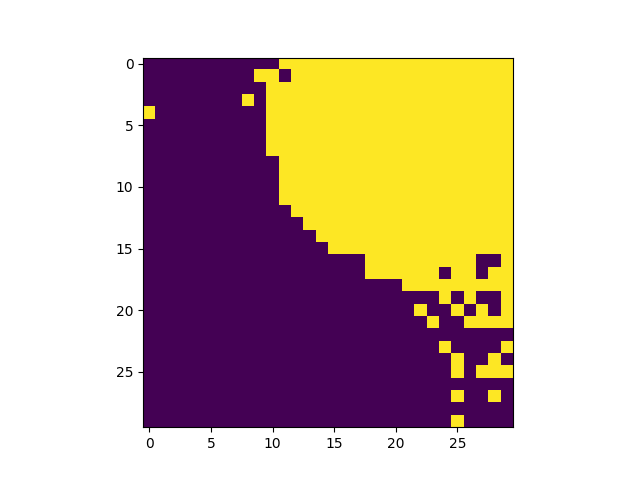
\includegraphics[width = 1.7in]{../figures/q2/som-training-04.png}} &
		\subfloat[Iteration 5]{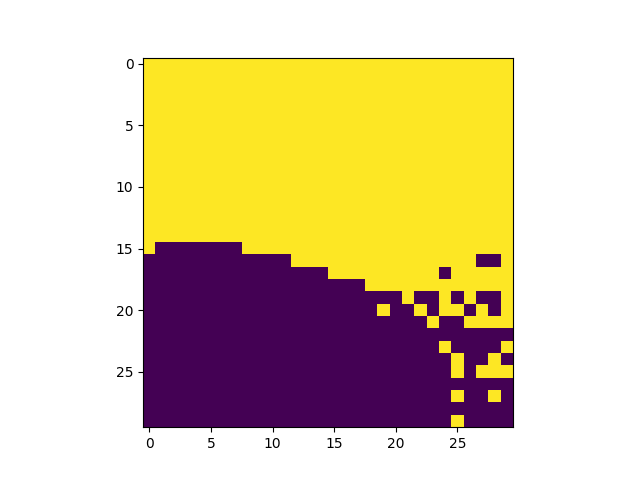
\includegraphics[width = 1.7in]{../figures/q2/som-training-05.png}} &
		\subfloat[Iteration 6]{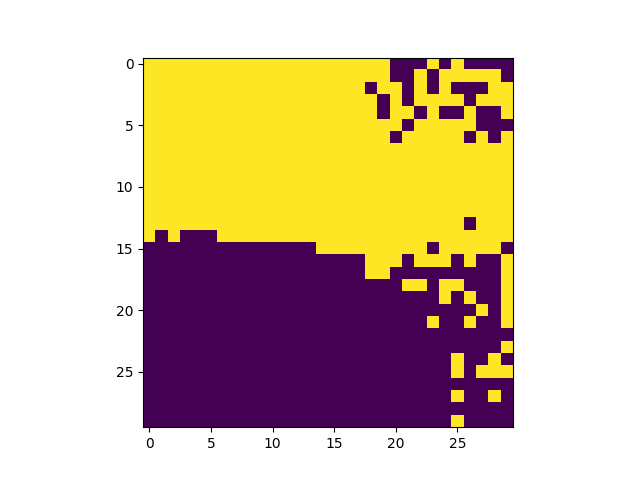
\includegraphics[width = 1.7in]{../figures/q2/som-training-06.png}} &
		\subfloat[Iteration 7]{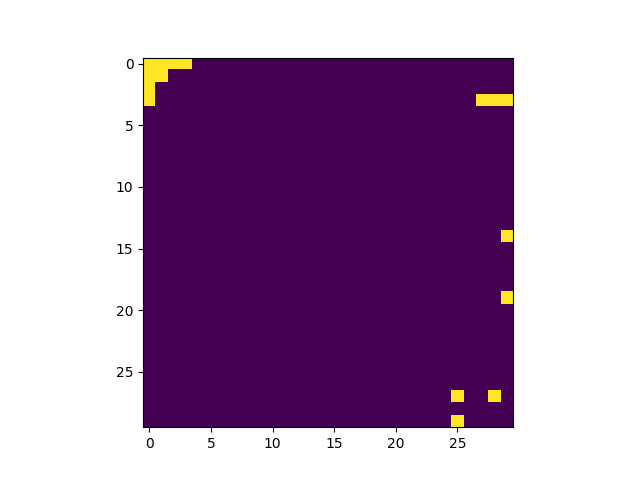
\includegraphics[width = 1.7in]{../figures/q2/som-training-07.png}}\\
		\subfloat[Iteration 8]{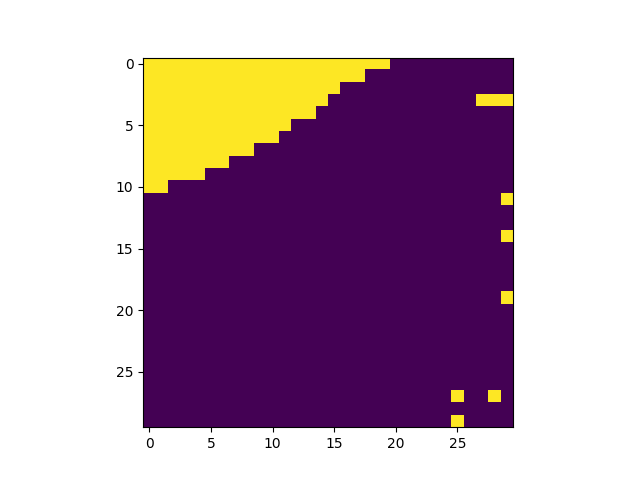
\includegraphics[width = 1.7in]{../figures/q2/som-training-08.png}} &
		\subfloat[Iteration 9]{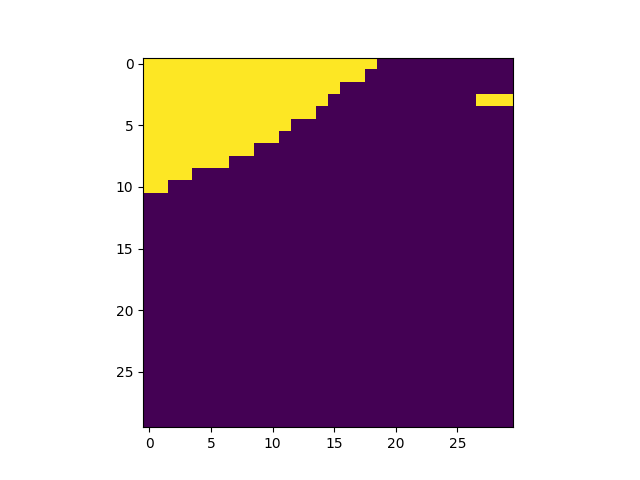
\includegraphics[width = 1.7in]{../figures/q2/som-training-09.png}} &
		\subfloat[Iteration 10]{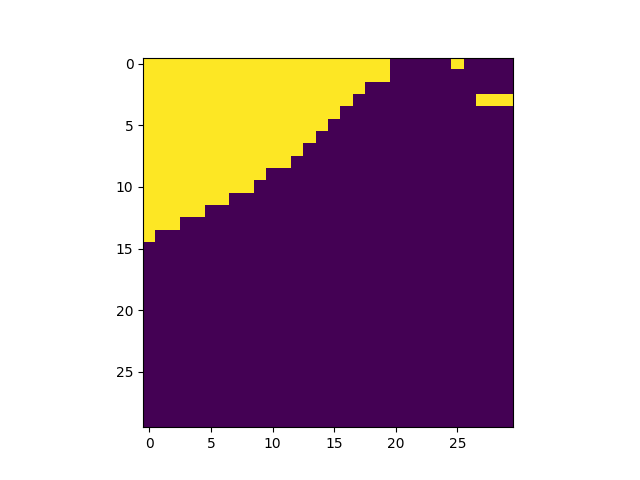
\includegraphics[width = 1.7in]{../figures/q2/som-training-10.png}} &
		\subfloat[Iteration 11]{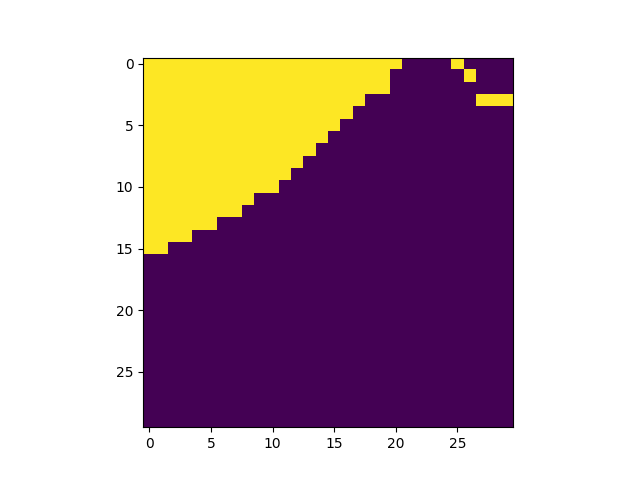
\includegraphics[width = 1.7in]{../figures/q2/som-training-11.png}}\\
		\subfloat[Iteration 12]{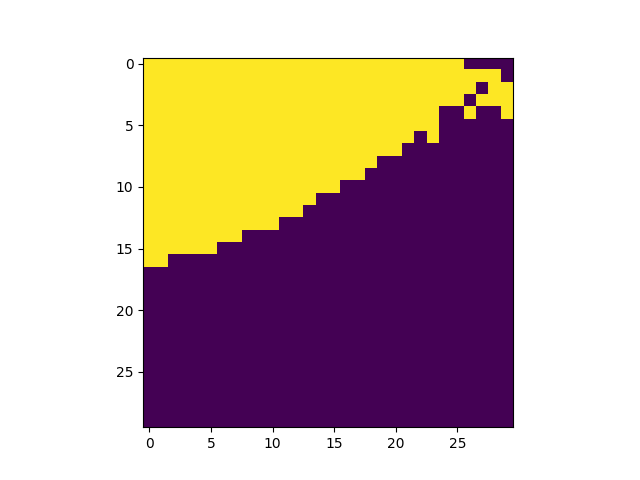
\includegraphics[width = 1.7in]{../figures/q2/som-training-12.png}} &
		\subfloat[Iteration 13]{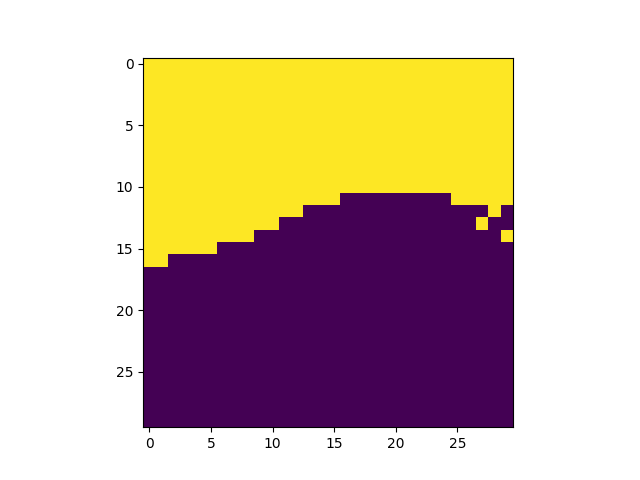
\includegraphics[width = 1.7in]{../figures/q2/som-training-13.png}} &
		\subfloat[Iteration 14]{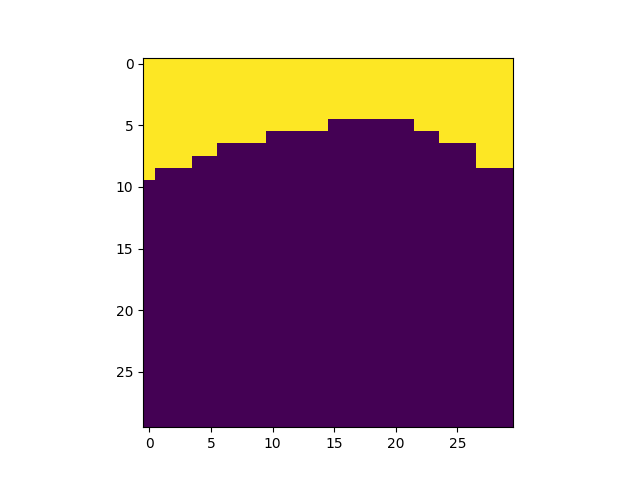
\includegraphics[width = 1.7in]{../figures/q2/som-training-14.png}} &
		\subfloat[Iteration 15]{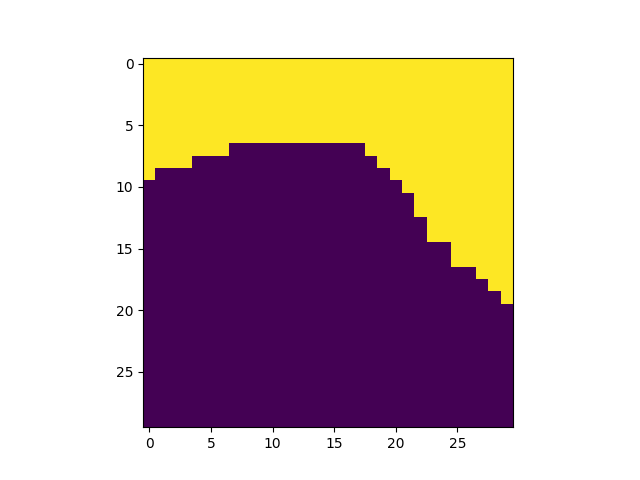
\includegraphics[width = 1.7in]{../figures/q2/som-training-15.png}}
	\end{tabular}
\end{figure}

\pagebreak

\subsubsection{SOM Output Neuron Prototypes}\label{som-output-neuron-prototypes}

We were interested in visualizing a few neurons' prototypes. A single
neuron's weights to the input later (784 weights in our case) represents
its prototype.
\\

The following charts visualize the prototypes of a few
randomly selected prototypes. Seeing these neat visualizations help us
be confident that our SOM is behaving correctly.

\begin{figure}[h!]
	\begin{tabular}{cc}
		\subfloat[Random Prototype \#1]{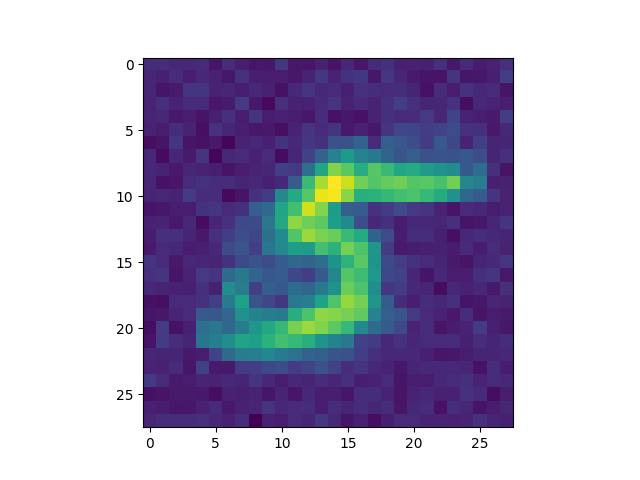
\includegraphics[width = 3.3in]{../figures/q2/neuron-prototype-01.png}} &
		\subfloat[Random Prototype \#2]{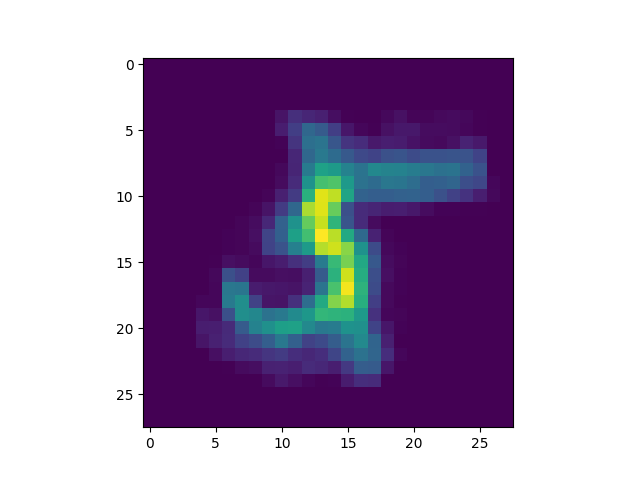
\includegraphics[width = 3.3in]{../figures/q2/neuron-prototype-02.png}}\\
		\subfloat[Random Prototype \#3]{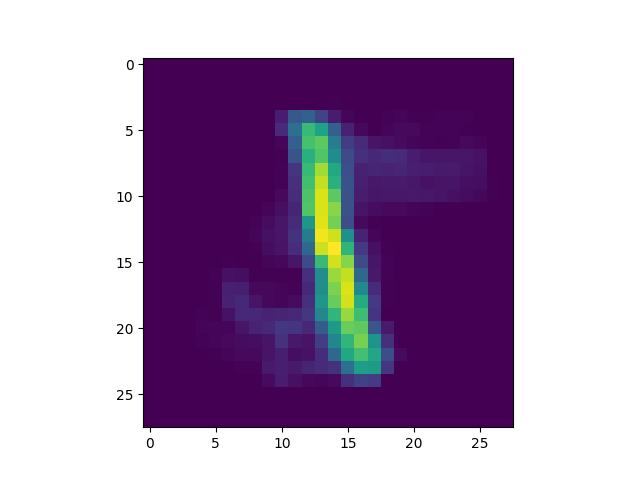
\includegraphics[width = 3.3in]{../figures/q2/neuron-prototype-03.png}} &
		\subfloat[Random Prototype \#4]{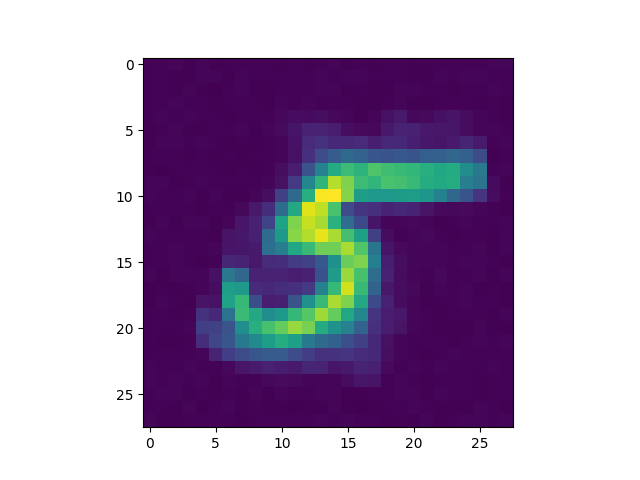
\includegraphics[width = 3.3in]{../figures/q2/neuron-prototype-04.png}}\\
		\subfloat[Random Prototype \#5]{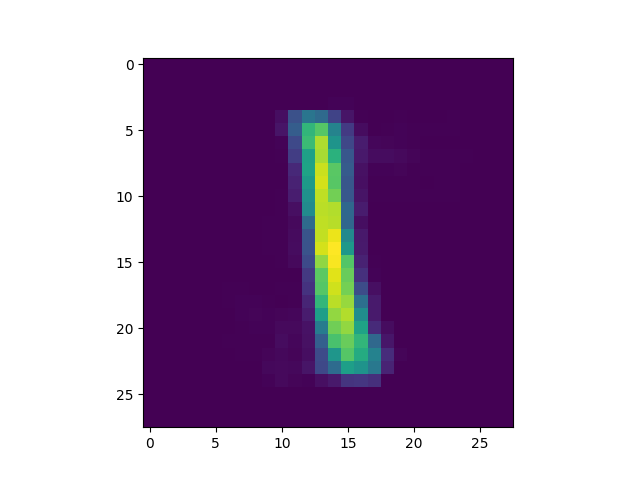
\includegraphics[width = 3.3in]{../figures/q2/neuron-prototype-05.png}} &
		\subfloat[Random Prototype \#6]{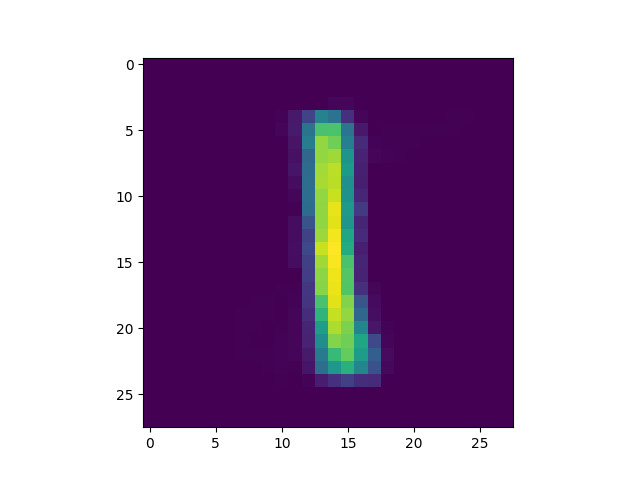
\includegraphics[width = 3.3in]{../figures/q2/neuron-prototype-06.png}}
	\end{tabular}
\end{figure}

\subsubsection{K-means Clustering}\label{k-means-clustering}

We wanted to keep the comparison between SOM "clustering" and K-means
clustering close, so we let \(k = 2\). After performing the K-means
clustering, we were able to tell if each element was correctly clustered
because we know the label for each MNIST image. We performed PCA on the
MNIST data to reduce it to 2 dimensions for visualization, as the
assignment specification suggests. Note that our use of PCA involves performing SVD,
which the assignment also suggested for this part of the assignment.
\\

This allowed us to
create the chart below, which indicated the elements that were clustered
correctly and those that were not. We also show the cluster centroids
computed by the K-means algorithm.

\begin{figure}[h!]
	\centering
	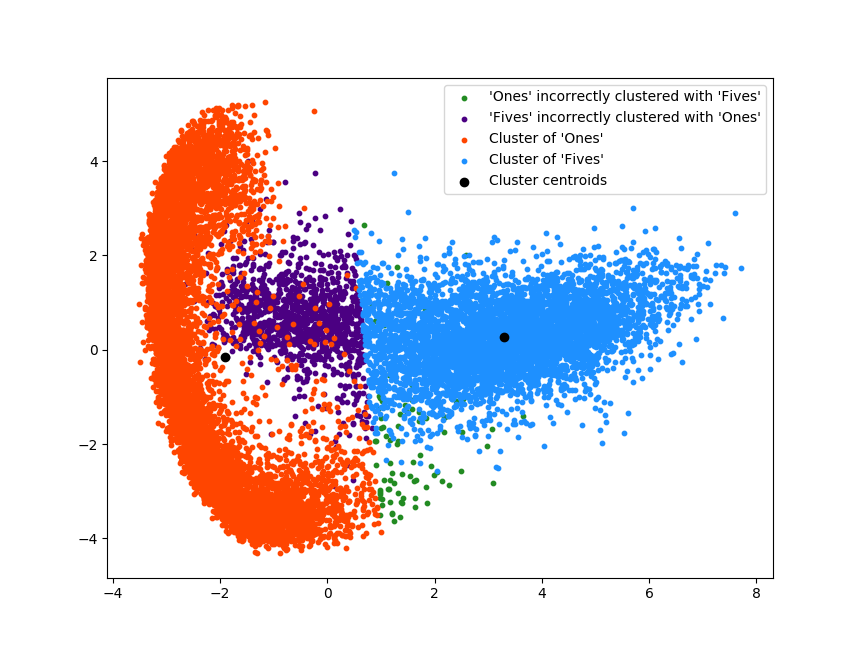
\includegraphics[scale=0.9]{../figures/q2/kmeans-clustering-small-dots.png}
	\caption{K-means Clustering of the MNIST Data Reduced to 2D}
\end{figure}

 \begin{center}\rule{0.5\linewidth}{\linethickness}\end{center}

\pagebreak


\section{Question 3}\label{question-3}

\subsection{Running Our Code}\label{running-our-code}

\textbf{Important:} our submission includes the LFW face data that our
program needs. We had to create a separate Python 2.7 utility obtain
this data because the scikit-learn tutorial requires PIL (an outdated,
little-supported) to read the data. We had to compile PIL from source,
so it's easier for us to include the data instead of making you manually
compile PIL and run \textit{yet} another script.
\\

We have provided an easy-to-use Makefile to help you run our program:

\begin{Verbatim}[frame=single,commandchars=\\\{\}]
    \PY{n}{make} \PY{n}{prepare}\PY{o}{\PYZhy{}}\PY{n}{venv}
    \PY{o}{.}\PY{o}{/}\PY{n}{env}\PY{o}{/}\PY{n+nb}{bin}\PY{o}{/}\PY{n}{python} \PY{n}{eigenfaces}\PY{o}{.}\PY{n}{py}      \PY{c+c1}{\PYZsh{} don\PYZsq{}t perform PCA on face data}
    \PY{o}{.}\PY{o}{/}\PY{n}{env}\PY{o}{/}\PY{n+nb}{bin}\PY{o}{/}\PY{n}{python} \PY{n}{eigenfaces}\PY{o}{.}\PY{n}{py} \PY{l+m+mi}{100}  \PY{c+c1}{\PYZsh{} perform PCA to obtain 100 components / eigenfaces}
\end{Verbatim}


    Otherwise, if you have tensorflow, matplotlib, numpy, and scikit-learn
installed already:

\begin{Verbatim}[frame=single,commandchars=\\\{\}]
    \PY{c+c1}{\PYZsh{} Syntax}
    \PY{n}{python3} \PY{n}{eigenfaces}\PY{o}{.}\PY{n}{py} \PY{p}{[}\PY{n}{num\PYZus{}PCA\PYZus{}components}\PY{p}{]}
    \PY{c+c1}{\PYZsh{} Example}
    \PY{n}{python3} \PY{n}{eigenfaces}\PY{o}{.}\PY{n}{py}      \PY{c+c1}{\PYZsh{} don\PYZsq{}t perform PCA on face data}
    \PY{n}{python3} \PY{n}{eigenfaces}\PY{o}{.}\PY{n}{py} \PY{l+m+mi}{100}  \PY{c+c1}{\PYZsh{} perform PCA to obtain 100 eigenfaces}
\end{Verbatim}


    Running the program will do the following:

\begin{enumerate}
	\def\labelenumi{\arabic{enumi}.}
	\tightlist
	\item Import the LFW face data from local files \textit{(provided with our submission)}.
	\item Perform 10-fold cross-validation; for each fold do:
	\begin{itemize}
		\tightlist
		\item Initialize a feed-forward network from scratch.
		\item Train the classifier on all 9 training folds for 100 epochs.
		\item After the final epoch, test for accuracy using the testing fold.
		\item Save the accuracy for this fold.
	\end{itemize}
	\item Compute the average accuracy over the 10 folds and print it out.
\end{enumerate}

\pagebreak

\subsection{Accuracy of Classification / Facial
Recognition}\label{accuracy-of-classification-facial-recognition}

First, we tested our feed-forward network with the face data to see how
well we can classify faces without the use of PCA. We performed 10-fold
cross validation, along with the following hyper-parameters:

\begin{Verbatim}[frame=single,commandchars=\\\{\}]
\PY{c+c1}{\PYZsh{} Hyper\PYZhy{}parameters}
\PY{n}{num\PYZus{}folds} \PY{o}{=} \PY{l+m+mi}{10}
\PY{n}{batch\PYZus{}size} \PY{o}{=} \PY{l+m+mi}{64}
\PY{n}{epochs} \PY{o}{=} \PY{l+m+mi}{100}
\PY{n}{learning\PYZus{}rate} \PY{o}{=} \PY{l+m+mf}{0.020}

\PY{c+c1}{\PYZsh{} Architecture (USED FOR ALL EXPERIMENTS)}
\PY{n}{input\PYZus{}neurons} \PY{o}{=} \PY{l+m+mi}{1850}    \PY{c+c1}{\PYZsh{} face images were 50x37 in size}
\PY{n}{hidden\PYZus{}neurons\PYZus{}1} \PY{o}{=} \PY{l+m+mi}{160}  \PY{c+c1}{\PYZsh{} hidden layer 1}
\PY{n}{hidden\PYZus{}neurons\PYZus{}2} \PY{o}{=} \PY{l+m+mi}{60}   \PY{c+c1}{\PYZsh{} hidden layer 2}
\PY{n}{output\PYZus{}neurons} \PY{o}{=} \PY{l+m+mi}{7}      \PY{c+c1}{\PYZsh{} dataset had faces of 7 unique people}
\end{Verbatim}


This yielded a classifier with \textbf{83.39\%} averaged cross-validated
accuracy.

We then applied PCA to the data before training on it, again using
10-fold cross-validation. We tried several values for the number of PCA
components (eigenfaces) to reduce the data to. \textbf{We used the exact
same architecture and hyper-parameters as the experiment on the raw face
data.} These experiments on the dimensionality-reduced datasets yielded
the cross-validated accuracy values in the chart below:

\subsubsection{Accuracy Chart}

\begin{figure}[h!]
	\centering
	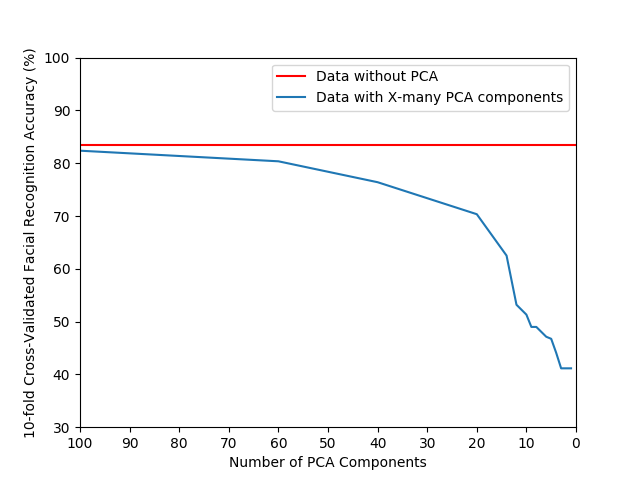
\includegraphics{../figures/q3/pca-accuracy.png}
	\caption{Classifier Accuracy: with and without PCA}
\end{figure}

\pagebreak

\subsubsection{Accuracy Chart Code}

\begin{Verbatim}[frame=single,commandchars=\\\{\}]
\PY{k+kn}{import} \PY{n+nn}{matplotlib}\PY{n+nn}{.}\PY{n+nn}{pyplot} \PY{k}{as} \PY{n+nn}{plt}
\PY{k+kn}{from} \PY{n+nn}{matplotlib}\PY{n+nn}{.}\PY{n+nn}{ticker} \PY{k}{import} \PY{n}{MaxNLocator}

\PY{n}{non\PYZus{}pca\PYZus{}accuracy} \PY{o}{=} \PY{l+m+mf}{83.39}

\PY{n}{num\PYZus{}eigenfaces} \PY{o}{=} \PY{p}{[}
    \PY{l+m+mi}{100}\PY{p}{,} \PY{l+m+mi}{60}\PY{p}{,} \PY{l+m+mi}{40}\PY{p}{,} \PY{l+m+mi}{20}\PY{p}{,}
     \PY{l+m+mi}{14}\PY{p}{,} \PY{l+m+mi}{12}\PY{p}{,} \PY{l+m+mi}{10}\PY{p}{,}  \PY{l+m+mi}{9}\PY{p}{,}
      \PY{l+m+mi}{8}\PY{p}{,}  \PY{l+m+mi}{7}\PY{p}{,}  \PY{l+m+mi}{6}\PY{p}{,}  \PY{l+m+mi}{5}\PY{p}{,}
      \PY{l+m+mi}{4}\PY{p}{,}  \PY{l+m+mi}{3}\PY{p}{,}  \PY{l+m+mi}{2}\PY{p}{,}  \PY{l+m+mi}{1}\PY{p}{,}
\PY{p}{]}
\PY{n}{pca\PYZus{}accuracy} \PY{o}{=} \PY{p}{[}
    \PY{l+m+mf}{82.37}\PY{p}{,} \PY{l+m+mf}{80.36}\PY{p}{,} \PY{l+m+mf}{76.40}\PY{p}{,} \PY{l+m+mf}{70.34}\PY{p}{,}
    \PY{l+m+mf}{62.50}\PY{p}{,} \PY{l+m+mf}{53.19}\PY{p}{,} \PY{l+m+mf}{51.32}\PY{p}{,} \PY{l+m+mf}{48.99}\PY{p}{,}
    \PY{l+m+mf}{48.99}\PY{p}{,} \PY{l+m+mf}{48.06}\PY{p}{,} \PY{l+m+mf}{47.13}\PY{p}{,} \PY{l+m+mf}{46.74}\PY{p}{,}
    \PY{l+m+mf}{44.10}\PY{p}{,} \PY{l+m+mf}{41.15}\PY{p}{,} \PY{l+m+mf}{41.15}\PY{p}{,} \PY{l+m+mf}{41.15}\PY{p}{,}
\PY{p}{]}

\PY{n}{fig} \PY{o}{=} \PY{n}{plt}\PY{o}{.}\PY{n}{figure}\PY{p}{(}\PY{p}{)}
\PY{n}{ax} \PY{o}{=} \PY{n}{fig}\PY{o}{.}\PY{n}{gca}\PY{p}{(}\PY{p}{)}

\PY{n}{plt}\PY{o}{.}\PY{n}{axhline}\PY{p}{(}\PY{n}{y}\PY{o}{=}\PY{n}{non\PYZus{}pca\PYZus{}accuracy}\PY{p}{,} \PY{n}{color}\PY{o}{=}\PY{l+s+s1}{\PYZsq{}}\PY{l+s+s1}{red}\PY{l+s+s1}{\PYZsq{}}\PY{p}{)}
\PY{n}{plt}\PY{o}{.}\PY{n}{plot}\PY{p}{(}\PY{n}{num\PYZus{}eigenfaces}\PY{p}{,} \PY{n}{pca\PYZus{}accuracy}\PY{p}{)}

\PY{n}{ax}\PY{o}{.}\PY{n}{xaxis}\PY{o}{.}\PY{n}{set\PYZus{}major\PYZus{}locator}\PY{p}{(}\PY{n}{MaxNLocator}\PY{p}{(}\PY{n}{integer}\PY{o}{=}\PY{k+kc}{True}\PY{p}{)}\PY{p}{)}
\PY{n}{plt}\PY{o}{.}\PY{n}{axis}\PY{p}{(}\PY{p}{[}\PY{l+m+mi}{100}\PY{p}{,} \PY{l+m+mi}{0}\PY{p}{,} \PY{l+m+mi}{30}\PY{p}{,} \PY{l+m+mi}{100}\PY{p}{]}\PY{p}{)}
\PY{n}{plt}\PY{o}{.}\PY{n}{xlabel}\PY{p}{(}\PY{l+s+s2}{\PYZdq{}}\PY{l+s+s2}{Number of PCA Components}\PY{l+s+s2}{\PYZdq{}}\PY{p}{)}
\PY{n}{plt}\PY{o}{.}\PY{n}{ylabel}\PY{p}{(}\PY{l+s+s2}{\PYZdq{}}\PY{l+s+s2}{10\PYZhy{}fold Cross\PYZhy{}Validated Facial Recognition Accuracy (}\PY{l+s+s2}{\PYZpc{}}\PY{l+s+s2}{)}\PY{l+s+s2}{\PYZdq{}}\PY{p}{)}
\PY{n}{plt}\PY{o}{.}\PY{n}{legend}\PY{p}{(}\PY{p}{[}\PY{l+s+s1}{\PYZsq{}}\PY{l+s+s1}{Data without PCA}\PY{l+s+s1}{\PYZsq{}}\PY{p}{,} \PY{l+s+s1}{\PYZsq{}}\PY{l+s+s1}{Data with X\PYZhy{}many PCA components}\PY{l+s+s1}{\PYZsq{}}\PY{p}{]}\PY{p}{,} \PY{n}{loc}\PY{o}{=}\PY{l+s+s1}{\PYZsq{}}\PY{l+s+s1}{upper right}\PY{l+s+s1}{\PYZsq{}}\PY{p}{)}

\PY{n}{plt}\PY{o}{.}\PY{n}{show}\PY{p}{(}\PY{p}{)}
\end{Verbatim}

\pagebreak

\subsection{Implementation}\label{implementation}

\subsubsection{Performing PCA}\label{performing-pca}

We used scikit-learn to perform PCA on the input face data:

\begin{Verbatim}[frame=single,commandchars=\\\{\}]
\PY{n}{num\PYZus{}components} \PY{o}{=} \PY{n+nb}{int}\PY{p}{(}\PY{n}{sys}\PY{o}{.}\PY{n}{argv}\PY{p}{[}\PY{l+m+mi}{1}\PY{p}{]}\PY{p}{)}
\PY{n}{pca} \PY{o}{=} \PY{n}{PCA}\PY{p}{(}\PY{n}{n\PYZus{}components}\PY{o}{=}\PY{n}{num\PYZus{}components}\PY{p}{,} \PY{n}{svd\PYZus{}solver}\PY{o}{=}\PY{l+s+s1}{\PYZsq{}}\PY{l+s+s1}{randomized}\PY{l+s+s1}{\PYZsq{}}\PY{p}{,} \PY{n}{whiten}\PY{o}{=}\PY{k+kc}{True}\PY{p}{)}\PY{o}{.}\PY{n}{fit}\PY{p}{(}\PY{n}{data}\PY{p}{)}
\PY{n}{data} \PY{o}{=} \PY{n}{pca}\PY{o}{.}\PY{n}{transform}\PY{p}{(}\PY{n}{data}\PY{p}{)}
\PY{n}{num\PYZus{}features} \PY{o}{=} \PY{n}{data}\PY{o}{.}\PY{n}{shape}\PY{p}{[}\PY{l+m+mi}{1}\PY{p}{]}
\end{Verbatim}


    \subsubsection{10-fold Cross-validation}\label{fold-cross-validation}

In our training process, our program performs the following: * for each
of the 10 folds: * initialize a feed-forward network from scratch *
train the classifier on all training folds for 100 epochs * after the
final epoch, save the accuracy using the testing fold * compute the
average accuracy over the 10 folds

\begin{Verbatim}[frame=single,commandchars=\\\{\}]
\PY{k}{for} \PY{n}{fold} \PY{o+ow}{in} \PY{n+nb}{range}\PY{p}{(}\PY{n}{num\PYZus{}folds}\PY{p}{)}\PY{p}{:}
    \PY{n+nb}{print}\PY{p}{(}\PY{l+s+s1}{\PYZsq{}}\PY{l+s+s1}{Using fold }\PY{l+s+si}{\PYZob{}:02d\PYZcb{}}\PY{l+s+s1}{ / }\PY{l+s+si}{\PYZob{}:02d\PYZcb{}}\PY{l+s+s1}{ as the training fold:}\PY{l+s+s1}{\PYZsq{}}\PY{o}{.}\PY{n}{format}\PY{p}{(}\PY{n}{fold} \PY{o}{+} \PY{l+m+mi}{1}\PY{p}{,} \PY{n}{num\PYZus{}folds}\PY{p}{)}\PY{p}{)}

    \PY{n}{train\PYZus{}indices}\PY{p}{,} \PY{n}{test\PYZus{}indices} \PY{o}{=} \PY{n}{folds}\PY{p}{[}\PY{n}{fold}\PY{p}{]}
    \PY{n}{trX}\PY{p}{,} \PY{n}{teX} \PY{o}{=} \PY{n}{data}\PY{p}{[}\PY{n}{train\PYZus{}indices}\PY{p}{]}\PY{p}{,} \PY{n}{data}\PY{p}{[}\PY{n}{test\PYZus{}indices}\PY{p}{]}
    \PY{n}{trY}\PY{p}{,} \PY{n}{teY} \PY{o}{=} \PY{n}{labels}\PY{p}{[}\PY{n}{train\PYZus{}indices}\PY{p}{]}\PY{p}{,} \PY{n}{labels}\PY{p}{[}\PY{n}{test\PYZus{}indices}\PY{p}{]}

    \PY{k}{with} \PY{n}{tf}\PY{o}{.}\PY{n}{Session}\PY{p}{(}\PY{p}{)} \PY{k}{as} \PY{n}{sess}\PY{p}{:}
        \PY{n}{tf}\PY{o}{.}\PY{n}{global\PYZus{}variables\PYZus{}initializer}\PY{p}{(}\PY{p}{)}\PY{o}{.}\PY{n}{run}\PY{p}{(}\PY{p}{)}
        \PY{k}{for} \PY{n}{epoch} \PY{o+ow}{in} \PY{n+nb}{range}\PY{p}{(}\PY{l+m+mi}{1}\PY{p}{,} \PY{n}{epochs} \PY{o}{+} \PY{l+m+mi}{1}\PY{p}{)}\PY{p}{:}
            \PY{n}{batch\PYZus{}starts} \PY{o}{=} \PY{n+nb}{range}\PY{p}{(}\PY{l+m+mi}{0}\PY{p}{,} \PY{n+nb}{len}\PY{p}{(}\PY{n}{trX}\PY{p}{)}\PY{p}{,} \PY{n}{batch\PYZus{}size}\PY{p}{)}
            \PY{n}{batch\PYZus{}ends} \PY{o}{=} \PY{n+nb}{range}\PY{p}{(}\PY{n}{batch\PYZus{}size}\PY{p}{,} \PY{n+nb}{len}\PY{p}{(}\PY{n}{trX}\PY{p}{)} \PY{o}{+} \PY{l+m+mi}{1}\PY{p}{,} \PY{n}{batch\PYZus{}size}\PY{p}{)}

            \PY{k}{for} \PY{n}{start}\PY{p}{,} \PY{n}{end} \PY{o+ow}{in} \PY{n+nb}{zip}\PY{p}{(}\PY{n}{batch\PYZus{}starts}\PY{p}{,} \PY{n}{batch\PYZus{}ends}\PY{p}{)}\PY{p}{:}
                \PY{n}{sess}\PY{o}{.}\PY{n}{run}\PY{p}{(}\PY{n}{train\PYZus{}op}\PY{p}{,} \PY{n}{feed\PYZus{}dict}\PY{o}{=}\PY{p}{\PYZob{}}\PY{n}{X}\PY{p}{:} \PY{n}{trX}\PY{p}{[}\PY{n}{start}\PY{p}{:}\PY{n}{end}\PY{p}{]}\PY{p}{,} \PY{n}{Y}\PY{p}{:} \PY{n}{trY}\PY{p}{[}\PY{n}{start}\PY{p}{:}\PY{n}{end}\PY{p}{]}\PY{p}{\PYZcb{}}\PY{p}{)}

            \PY{k}{if} \PY{n}{epoch} \PY{o}{\PYZpc{}} \PY{l+m+mi}{20} \PY{o}{==} \PY{l+m+mi}{0}\PY{p}{:}
                \PY{n}{epoch\PYZus{}accuracy} \PY{o}{=} \PY{n}{np}\PY{o}{.}\PY{n}{mean}\PY{p}{(}\PY{n}{np}\PY{o}{.}\PY{n}{argmax}\PY{p}{(}\PY{n}{teY}\PY{p}{,} \PY{n}{axis}\PY{o}{=}\PY{l+m+mi}{1}\PY{p}{)} \PY{o}{==} \PY{n}{sess}\PY{o}{.}\PY{n}{run}\PY{p}{(}\PY{n}{predict\PYZus{}op}\PY{p}{,} \PY{n}{feed\PYZus{}dict}\PY{o}{=}\PY{p}{\PYZob{}}\PY{n}{X}\PY{p}{:} \PY{n}{teX}\PY{p}{\PYZcb{}}\PY{p}{)}\PY{p}{)}
                \PY{n+nb}{print}\PY{p}{(}\PY{l+s+s1}{\PYZsq{}}\PY{l+s+se}{\PYZbs{}t}\PY{l+s+s1}{Epoch }\PY{l+s+si}{\PYZob{}:3\PYZcb{}}\PY{l+s+s1}{ \PYZhy{}\PYZhy{}\PYZhy{}\PYZgt{} }\PY{l+s+si}{\PYZob{}:.2f\PYZcb{}}\PY{l+s+s1}{\PYZpc{}}\PY{l+s+s1}{\PYZsq{}}\PY{o}{.}\PY{n}{format}\PY{p}{(}\PY{n}{epoch}\PY{p}{,} \PY{n}{epoch\PYZus{}accuracy} \PY{o}{*} \PY{l+m+mi}{100}\PY{p}{)}\PY{p}{)}

    \PY{n}{fold\PYZus{}accuracy}\PY{o}{.}\PY{n}{append}\PY{p}{(}\PY{n}{epoch\PYZus{}accuracy}\PY{p}{)}
    \PY{n+nb}{print}\PY{p}{(}\PY{l+s+s1}{\PYZsq{}}\PY{l+s+s1}{Accuracy with fold \PYZsh{}}\PY{l+s+si}{\PYZob{}\PYZcb{}}\PY{l+s+s1}{ as training: }\PY{l+s+si}{\PYZob{}:.2f\PYZcb{}}\PY{l+s+s1}{\PYZpc{}}\PY{l+s+se}{\PYZbs{}n}\PY{l+s+s1}{\PYZsq{}}\PY{o}{.}\PY{n}{format}\PY{p}{(}\PY{n}{fold} \PY{o}{+} \PY{l+m+mi}{1}\PY{p}{,} \PY{n}{fold\PYZus{}accuracy}\PY{p}{[}\PY{o}{\PYZhy{}}\PY{l+m+mi}{1}\PY{p}{]} \PY{o}{*} \PY{l+m+mi}{100}\PY{p}{)}\PY{p}{)}

\PY{n}{accuracy} \PY{o}{=} \PY{n+nb}{sum}\PY{p}{(}\PY{n}{fold\PYZus{}accuracy}\PY{p}{)} \PY{o}{/} \PY{n+nb}{len}\PY{p}{(}\PY{n}{fold\PYZus{}accuracy}\PY{p}{)}
\PY{n+nb}{print}\PY{p}{(}\PY{l+s+s1}{\PYZsq{}}\PY{l+s+s1}{Average }\PY{l+s+si}{\PYZob{}\PYZcb{}}\PY{l+s+s1}{\PYZhy{}fold cross validation accuracy: }\PY{l+s+si}{\PYZob{}:.2f\PYZcb{}}\PY{l+s+s1}{\PYZpc{}}\PY{l+s+s1}{\PYZsq{}}\PY{o}{.}\PY{n}{format}\PY{p}{(}\PY{n}{num\PYZus{}folds}\PY{p}{,} \PY{n}{accuracy} \PY{o}{*} \PY{l+m+mi}{100}\PY{p}{)}\PY{p}{)}
\end{Verbatim}

\begin{center}\rule{0.5\linewidth}{\linethickness}\end{center}

\pagebreak

\section{References}\label{references}

\subsection{Question 1}\label{question-1}

\begin{itemize}
\item
  https://en.wikipedia.org/wiki/Hopfield\_network
\item
  http://citeseerx.ist.psu.edu/viewdoc/download?doi=10.1.1.33.103\&rep=rep1\&type=pdf
  \textit{(Storkey's paper)}
\end{itemize}

\subsection{Question 2}\label{question-2}

\begin{itemize}
\item
  https://github.com/JustGlowing/minisom
\item
  https://en.wikipedia.org/wiki/Self-organizing\_map
\end{itemize}

\subsection{Question 3}\label{question-3}

\begin{itemize}
\item
  We used the TensorFlow feed-forward code from our in-class tutorials.
\item
  http://scikit-learn.org/stable/modules/generated/sklearn.model\_selection.KFold.html
\item
  http://scikit-learn.org/0.18/auto\_examples/applications/face\_recognition.html
\end{itemize}

\begin{center}\rule{0.5\linewidth}{\linethickness}\end{center}

\end{document}
